% thesis.tex
%
% This file is root file for an example thesis written using the
% IIT Bombay LaTeX Style file.
% Created by Amey Karkare (21 June 2007)
%
% It is provided without warranty on an AS IS basis.

%=====================================================================
% Read: http://www.cse.iitb.ac.in/karkare/iitbthesis/
%    FAQ.txt     for frequently asked quetions
%    Changes.txt for changes
%    README      for more information
%=====================================================================

%=====================================================================
% DOCUMENT STYLE
%=====================================================================
% IITB PhD Thesis format default settings are:
%   12pt, one-sided printing on a4 size paper
\documentclass[openright,twoside]{iitkthesis}
% For two-sided printing, with Chapter starting on odd-numbered pages,
% use the following line instead:  
%%\documentclass[openright,twoside]{iitbthesis}

%=====================================================================
% OPTIONAL PACKAGES
%=====================================================================
% To include optional packages, use the \usepackage command.
% For e.g., The package epsfig is used to bring in the Encapsulated
%    PostScript figures into the document.
%    The package times is used to change the fonts to Times Roman;
%=====================================================================

%=====================================================================
%  Single counter for theorems and theorem-like environments:
%=====================================================================
\newtheorem{theorem}{Theorem}[chapter]
\newtheorem{assertion}[theorem]{Assertion}
\newtheorem{claim}[theorem]{Claim}
\newtheorem{conjecture}[theorem]{Conjecture}
\newtheorem{corollary}[theorem]{Corollary}
\newtheorem{definition}[theorem]{Definition}
\newtheorem{example}[theorem]{Example}
\newtheorem{figger}[theorem]{Figure}
\newtheorem{lemma}[theorem]{Lemma}
\newtheorem{prop}[theorem]{Proposition}
\newtheorem{remark}[theorem]{Remark}

\usepackage{etex}
\usepackage{minted}
\usemintedstyle{bw}

\usepackage{fontspec}
\setmonofont[Scale=0.85]{DejaVu Sans Mono}

\usepackage[backend=biber, sorting=none]{biblatex}
\usepackage{amsmath}
\usepackage{lipsum}
\usepackage{float}
\usepackage[hidelinks]{hyperref}
\usepackage{microtype}
\usepackage[font=small,labelfont=bf]{caption}
\usepackage{fancyref}
\usepackage{color,soul} % for highlights
\usepackage{enumerate}
\usepackage{tabularx}
\usepackage{mathabx}
\usepackage{algorithm}
\usepackage{algpseudocode}
\usepackage{graphicx}
\usepackage{gb4e}

\setcounter{secnumdepth}{3}

\renewcommand{\algorithmicrequire}{\textbf{Require:}}
\renewcommand{\algorithmicensure}{\textbf{Ensure:}}

\graphicspath{ {images/} }

\setlength{\headheight}{15pt}

\expandafter\def\csname PY@tok@err\endcsname{}

\floatstyle{ruled}
\newfloat{program}{thp}{lop}
\floatname{program}{Figure}

\numberwithin{program}{chapter}

\BeforeBeginEnvironment{program}{\begin{singlespace}}
\AfterEndEnvironment{program}{\end{singlespace}}
\bibliography{citations}

%=====================================================================
% End of Preamble, start of document
%

\begin{document}

%=====================================================================
% Include the prelude for Title page, abstract, table of contents, etc
% You need to modify it to contain your details
% prelude.tex
%   - titlepage
%   - dedication (optional)
%   - approval sheet
%   - course certificate
%   - table of contents, list of tables and list of figures
%   - nomenclature
%   - abstract
%============================================================================


\clearpage\pagenumbering{roman}  % This makes the page numbers Roman (i, ii, etc)



% TITLE PAGE
%   - define \title{} \author{} \date{}
\title{A Tool for Teaching Parsing Techniques}
\author{Nimisha Agarwal}
\date{July, 2015}

%  - Roll number, required for title page, approval sheet, and
%    certificate of course work 
\rollnum{13111038} 

%   - The default degree is ``Doctor of Philosophy''
%     (unless the document style msthesis is specified
%      and then the default degree is ``Master of Science'')
%     Degree can be changed using the command \iitbdegree{}
\iitbdegree{Master of Technology}

%   - The default report type is preliminary report.
%      * for a PhD thesis, specify \thesis
\thesis
%      * for a M.Tech./M.Phil./M.Des./M.S. dissertation, specify \dissertation
%\dissertation
%      * for a DIIT/B.Tech./M.Sc.project report, specify \project
%\project
%      * for any other type, use  \reporttype{}
%\reporttype{ReportType}

%   - The default department is ``Unknown Department''
%     The department can be changed using the command \department{}
\department{Computer Science \& Engineering}

%    - Set the guide's name
\setguide{Prof Amey Karkare}
\setguidedept{Department of Computer Science \& Engineering}

%   - once the above are defined, use \maketitle to generate the titlepage
\maketitle

%--------------------------------------------------------------------%
% CERTIFICATE
%     The first page after the title page.
\makecertificate

%--------------------------------------------------------------------%
% COPYRIGHT PAGE
%   - To include a copyright page use \copyrightpage
% \copyrightpage

%--------------------------------------------------------------------%
% ABSTRACT
\begin{abstract}
Interactive Educational Systems is an emerging field in today's world. It compensates the drawbacks of traditional classroom based education by making courses more reachable and manageable. Students are able to absorb knowledge at their own pace and time, rather than synchronize with the speed of instruction in classrooms. 

In this thesis, we have developed an tool for teaching the parsing phase of Compilers. The tool tries to impart knowledge of various parsing techniques to users through generated problems and hints. Problems are generated based on a Context Free Grammar (CFG) given as input. The tool evaluates these generated problems upon receiving the solutions to these problems from the users. Upon evaluation, it generates hint questions when the solutions provided by the users are incorrect. The problems follow a general Multiple Choice Question (MCQ) pattern, where a user is given a problem with a set of possible choices. The hint question generation procedures involve different sorts of algorithms, of which the input string generation algorithm is notable. This algorithm enables creation of an input string based on an incorrect answer provided by the user. Features of this sort help users to learn concepts in parsing in better depth, by understanding the mistakes that they commit.
\end{abstract}

%--------------------------------------------------------------------%
% DEDICATION
%   Dedications, if any.
\begin{dedication}
To my parents
\end{dedication}

% Acknowledgements
\begin{acknowledgments}

I would like to express my gratitude towards my thesis supervisor Prof. Amey Karkare, for providing me his valuable guidance and support throughout this thesis work. It would not have been possible to complete this thesis in due time and come up with an effective tool without his aid. He has provided me with the necessary resources to gather knowledge on building tools for programming languages and compilers. He has also enlightened me on solutions to problems which seemed too difficult to solve for me. I am highly thankful for all the motivation that he has provided to accomplish the thesis work.

I would also like to thank Mohit Bhadade for creating a web-based graphical user interface for the tool developed in this thesis. This has made it possible to demonstrate the real-world capabilities of the tool, by making it usable by students.

\end{acknowledgments}

%--------------------------------------------------------------------%
% CONTENTS, TABLES, FIGURES
\tableofcontents
\listofalgorithms
\addcontentsline{toc}{chapter}{List of Algorithms}

\cleardoublepage
%\phantomsection \label{listoffig}
\listoffigures

\cleardoublepage\pagenumbering{arabic} % Make the page numbers Arabic (1, 2, etc)


%=====================================================================
% Include the technical part of the report
%% \include{chap_intro}             % Chapter 1: Introduction
%% \include{chap_others}            % Other chapters as required
%% \include{chap_conclusions}       % Finally the summary & conclusions

%=====================================================================
% APPENDIX
%  Appendices, if any, must precede the cited literatures.
%  Appendices shall be numbered in Roman Capitals (e.g. Appendix IV)

%% \appendix
%% \include{appendix_something}          

%=====================================================================
% PUBLICATIONS
%  publications if any may be listed after the literature cited.
%% \include{mypubs}

%=====================================================================
% ACKNOWLEDGMENTS
%   This is the last item in the thesis. It should be signed by
%   author, with date.


\chapter{Introduction}
\label{chap:intro}

Interactive Educational Systems is an emerging technology nowadays. It started with school level education for courses like Maths, English, etc. Presently interactive courses are available for many technical and advanced studies. 

In earlier times, classroom teaching was the only way to impart education. It has been an effective mode of education for several ages, but it has constraints. There are always students in a class who are not able to interact much with their professors or classmates. Classroom education is restricted to a particular physical location, so it is not available to a significantly large audience. Above that, classrooms are generally conducted for a limited time and hence it is not possible to solve all the queries or doubts of students, then and there.

Now, an alternative method is evolving to solve the problems of classroom education. Interactive Educational Systems are generally interactive in nature. Students can be provided with questions for practice which can be evaluated by the system itself. This reduces the overhead of instructor and hence allows accommodation of a large number of students in the course. Problems can also be generated by such systems. Some systems also provide feedback to the students after evaluating their answers.

In this thesis, we propose an Interactive Educational System for the parsing phase of Compilers. The results of the tool developed during the thesis work have been detailed in Chapter \ref{chap:interactions}.

\section{Objective}
\label{objective}
The purpose of this Thesis is to create an Interactive Tutoring System for the parsing phase of Compilers. The main objective is to generate problems automatically and evaluate the solution to those problems, which are submitted by the students. If a solution is wrong, then the system generates hint problems which guide the student to reach to the correct solution to the main problem. Otherwise it generates the next main problem. This work-flow is accomplished by calculating the solution to the problem beforehand. This pre-computed solution is then compared with the solution given by the student. The goal of this thesis is to generate problems automatically and provide immediate feedback to the students, while solving problems. 

\section{Motivation of Work}
\label{motivation}
Students generally face a lot of problems in learning compiler technology. They do not understand the different techniques involved in various phases of program compilation. Parsing is one of such phases, which consists of a large number of techniques. Students face many problems in grasping these techniques.

Parsing techniques mostly follow different algorithms to solve a parsing problem. This requires a step by step method to reach to the solution to such a problem. If a student makes a mistake in even one step, then the result is completely wrong. It is also very difficult for the student or the instructor to figure out such a mistake as it involves recalculation of all the steps.

Therefore, we needed a system that can provide students with a large number of problems for practice. We also needed to make them realise their mistakes by generating feedback. Feedback is a necessary step to guide a student to the correct solution. Our feedback provide students with hint questions of different types to make them understand what went wrong and how to reach to the correct solution.

\section{Outline of the Solution}
\label{outline}
The system is divided into three parts. Figure 1.1 gives an abstract view of the system.
\begin{figure}[h]
\centering
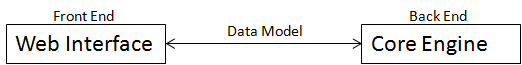
\includegraphics{Figure1.png}
\caption{Framework of the System}
\label{fig:framework}
\end{figure}

The system is mainly consists of:
\begin{itemize}
\item \textbf{Core Engine:} This part of the system deals with generation of problems, evaluation the answers given by students and generating hint questions automatically based on the answer given by students.
\item \textbf{Data Model:} It acts as an interface between front-end and back-end. It is used to transfer data back-and-forth between core engine and web interface.
\item \textbf{Web Interface:} This part provides a user-friendly environment to the student. It deals with the presentation of problems and provides ease of giving solutions.
\end{itemize}

\section{Contribution of Thesis}
\label{contribution}
In this thesis, we have implemented a tool for the parsing phase of compilers. It generates problems automatically for the different techniques involved in this phase, i.e. First set, Follow set, LL Parsing (which includes LL Parsing Table and LL Parsing Moves) and SLR Parsing (which includes SLR Canonical set, SLR Parsing Table and SLR Parsing Moves). We have tested the system on various grammars. The system also includes functionality like generation of input strings for a particular cell of the LL Parsing Table (in which a student has made a wrong entry while filling the table) and showing LL Parsing moves on that string to make the student understand, why the value she entered in the cell is incorrect.

\section{Thesis Organization}
\label{organization}
Rest of the thesis is organised as follows:

\textbf{Chapter 2} covers the background knowledge required to understand this thesis. It covers concepts from compiler technology, with additional stress on parsing techniques. 

\textbf{Chapter 3} presents an overview of the tool developed during the thesis work. It describes the architecture of the tool along with the various phases in the workflow of the tool. A few examples are also included to provide a better understanding of the concepts and the algorithms used in the tool.

\textbf{Chapter 4} contains all the major algorithms required to build the educational tool. The procedures for problem generation in each of the covered domains have been described here through the use of plain English and pseudo-code illustrations. Wherever necessary, examples and figures have also been included to provide a better understanding of the procedures.

\textbf{Chapter 5} captures the interface exported by the tool. This interface is required to enable the tool to be used via a graphical user interface, for effectiveness of instruction. The chapter covers the description of the files used to perform this integration.

\textbf{Chapter 6} illustrates the working of the tool through the use of narrations and screenshots. It covers an interactive walkthrough of the tool.
\chapter{Background}
\label{chap:background}
This chapter provides an overview of the concepts required to understand this thesis. Brief explanations about concepts in Compiler Design are covered here~\cite{aho1977principles}.

\section{Compiler}
\label{sec:compiler}
A translator is a program that converts a program written in one programming language (the source language) into a program in another language (the object or target language). A compiler is a translator, whose source language is a high-level programming language (such as C, C++), and object language is a low-level language such as assembly language or machine language.

The compilation process is divided into 5 phases as shown in Figure \ref{fig:Compiler Phases}.
\begin{figure}
\centering
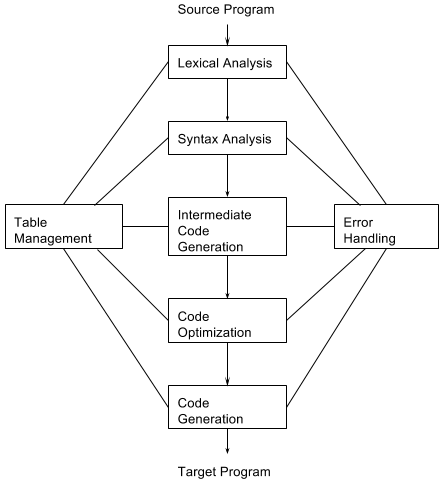
\includegraphics[width=1\textwidth]{CompilerPhases.png}
\caption{Phases of Compiler}
\label{fig:Compiler Phases}
\end{figure}

Following is a brief description of each of the phases of a Compiler:
\begin{enumerate}
\item \textbf{Lexical Analysis:} The first phase of Compiler is called Lexical Analysis. The tool (lexical analyzer or scanner) built for this task, separates the characters of the source language into groups that logically belong together. These groups are called tokens.

The usual tokens are:
\begin{itemize}
\item \textbf{Keywords:} Keywords are the reserved words in a programming language. They have the fixed meaning and cannot be changed by the user. Examples include 'IF', 'WHILE', etc.
\item \textbf{Identifiers:} These are the variables and function names defined by the user in the program, such as 'x', 'sum'.
\item \textbf{Operator Symbols:} They symbolize a specific action and operate on certain values. Examples include '<', '+', etc.
\item \textbf{Punctuation Symbols:} They separates words or phrases (that have meaning to a compiler). Examples include '(', ',', etc.
\end{itemize}
The output of this phase is a stream of tokens, which is passed to the next phase of Compiler.

\item \textbf{Syntax Analysis:} The syntax analyzer or parser groups tokens together into syntactic structures. If A*B+C is a string (containing 5 tokens), then it can be considered as (A*B)+C or as A*(B+C), depending on the language definition. The syntactic structure determines how these tokens are to be grouped together into larger structures called syntactic categories such as: \textbf{expressions} - sequences of operator and operands (constants and identifiers) or \textbf{statements} - multiple expressions can be combined to form statements.

The syntactic structure can be represented as a tree, known as a parse tree. Tokens appear on the leaves of this tree and the interior nodes of the tree represent strings of tokens that logically belong together.
\begin{example}
The three tokens representing 'A+B' can be grouped into an expression. The parse tree for 'A+B' can be represented as in Figure \ref{fig:SyntaxTree}.
\begin{figure}
\centering
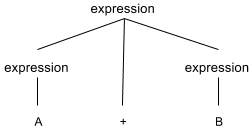
\includegraphics[width=0.5\textwidth]{SyntaxTree.png}
\caption{Parse Tree for A+B}
\label{fig:SyntaxTree}
\end{figure}
\end{example}

\item \textbf{Intermediate Code Generation:} The intermediate code generator uses the structure produced by the syntax analyzer to create a stream of simple instructions. These instructions can be in the form of "Macros".

\textbf{Macros} are small functions which can be converted into assembly language code.
\begin{example}
For addition, a macro can be defined as:
\begin{minted}{C}
MACRO   ADD2    X,Y
        LOAD    Y
        ADD     X
        STORE   Y
ENDMACRO
\end{minted}
For A+B, this macro can be used as:
\begin{minted}{C}
LOAD    B
ADD     A
STORE   B
\end{minted}
\end{example}

\item \textbf{Code Optimization:} This phase is used to improve the intermediate code so that the final object program runs faster and/or takes less space. Its output is another intermediate code program which is an improved version of the previous one.
\begin{example}
Suppose we have the following code snippet:
\begin{minted}{Java}
while(j<=10)
{
    i = 2;
    j = j + i;
}
\end{minted}

Here, the assignment i = 2 is executed in every iteration of the loop. But, the value of i remains constant in all iterations and is not changed in the loop. So, this assignment statement can be placed outside the loop to optimize the code such as
\begin{minted}{Java}
i = 2;
while(j<=10)
{
    j = j + i;
}
\end{minted}
\end{example}

\item \textbf{Code Generation:} This is the final phase of Compiler. It produces the object code by deciding on the memory locations for data, selecting code to access each datum, and selecting the registers in which each computation is to be done.
\begin{example}
For the instruction "A+B", code can be generated as:
\begin{minted}{C}
MOV A, R0
ADD B, R0
\end{minted}
\end{example}

\item \textbf{Table Management:} Table Management or book-keeping keeps track of the names used by the program and records essential information about each. An example of information is the type (integer, real) of a variable. For storing such information a data structure known as a symbol table is used.

\item \textbf{Error Handling:} The error handler warns the programmer about the flaws in the source program, by issuing a diagnostic and adjusting the information being passed from phase to phase, so that compilation can proceed till the last phase.
\end{enumerate}

\subsection{Some Terminology}
\label{subsec:Terminology}
Some terms related to the parsing phase of Compiler have been used in this thesis. A brief description of these terms is given below:
\begin{itemize} %add ref{https://en.wikipedia.org/wiki/Formal_grammar}
\item \textbf{Alphabet:} The set of symbols used in a programming language is called the alphabet of that programming language. Eg: \{a,b\}.
\item \textbf{Language:} Any set of strings formed from some specific alphabet. Eg: L = \{\{$\epsilon$, a, b, aa, bb, ab, ba\} | \{a,b\} $\in$ alphabet\}.
\item \textbf{Kleene Closure:} It is a unary operation defined as follows: if V is a set of symbols or characters, then V* (kleene closure) is the set of all strings over symbols in V, including the empty string $\epsilon$.
\item \textbf{Grammar:} A grammar is a set of production rules, to form strings from a language's alphabet. A grammar checks the validity of strings, by checking their syntactic correctness.

A grammar G = (N, $\Sigma$, P, S) consists of the following components:
\begin{itemize}
\item A finite set \textbf{N} of non-terminals (synonym for syntactic categories), that is disjoint with the strings formed from G.
\item A finite set \textbf{$\Sigma$} of terminals (synonym for tokens) that is disjoint from N.
\item A finite set \textbf{P} of production rules, each rule of the form \\
 $(\Sigma \cup N)^{*} N (\Sigma \cup N)^{*} \rightarrow (\Sigma \cup N)^{*}$ \\
where * is the Kleene closure and $\cup$ denotes set union.
\item The symbol \textbf{S}, where S $\in$ N is the start symbol.
\end{itemize}

\begin{example}
The grammar G, where N = $\left \{S, B\right \}$, $\Sigma = \left \{a, b, c\right \}$, S is the start symbol, and P consists of the following production rules:
\item $S \rightarrow aBSc$
\item $S \rightarrow abc$
\item $Ba \rightarrow aB$
\item $Bb \rightarrow bb$
\end{example}

\item \textbf{Context-free Grammar:} A context-free grammar(CFG) is a grammar in which the left-hand side of each production rule consists of only a single non-terminal symbol.
\begin{example}
\label{ex:CFG}
The grammar with N = $\left \{S\right \}$, $\Sigma=\left \{a,b\right \}$, S the start symbol, and the following production rules, P:
\item $S \rightarrow aSb$
\item $S \rightarrow ab$
\end{example}

\item \textbf{Derivation:} A derivation replaces a non-terminal on the LHS of a production with its respective RHS.
\begin{example}
One of the strings, which can be derived from the grammar in example \ref{ex:CFG}, by the following steps:

$S \Rightarrow aSb \Rightarrow aaSbb \Rightarrow aaabbb$
\end{example}
If the leftmost non-terminal is always expanded in the derivation, to acquire the string, then it is a leftmost derivation. Similarly if  the rightmost non-terminal is always expanded, then it is a rightmost derivation.
\begin{example}
Suppose the grammar is:
\begin{eqnarray*}
E&\rightarrow& T\ E'\\
E'&\rightarrow& +\ E \\
  & \mid& \epsilon\\
T&\rightarrow&0
\end{eqnarray*}

then, the following is the leftmost derivation

$E \Rightarrow TE' \Rightarrow 0E' \Rightarrow 0+E \Rightarrow 0+TE' \Rightarrow 0+0E' \Rightarrow 0+0$

and the rightmost derivation can be

$E \Rightarrow TE' \Rightarrow T+E \Rightarrow T+TE' \Rightarrow T+T \Rightarrow T+0 \Rightarrow 0+0$
\end{example}

\item \textbf{Sentential Form:} Let G = (N, $\Sigma$, P, S) be a CFG, and $\alpha\in(N\cup\Sigma)^*$. If $S\overset{*}{\Rightarrow}\alpha$ (where $\overset{*}{\Rightarrow}$ means derivation in zero or more steps), then $\alpha$ is the sentential form.

If $S\underset{lm}{\Rightarrow}\alpha$ (leftmost derivation), then $\alpha$ is a left-sentential form and if $S\underset{rm}{\Rightarrow}\alpha$ (rightmost derivation), then $\alpha$ is a right-sentential form.
%add ref http://www.univ-orleans.fr/lifo/Members/Mirian.Halfeld/Cours/TLComp/res1-CG.pdf
\begin{example}
Consider the example \ref{ex:CFG}. Each of \{S, aSb, aaSbb, aaabbb\}, derived from the set of production rules, is a sentential form.
\end{example}

\item \textbf{Lookahead:} Some parsing algorithms use a technique of looking ahead certain tokens in order to decide which rule to use. The maximum number of tokens that a parser can use to decide which rule it should use, is known as lookahead. % add ref https://en.wikipedia.org/wiki/Lookahead

\item \textbf{Handle:} A handle of a string is a substring that matches the right side of a production and whose reduction to the non-terminal on the left side of the production represents one step along the reverse of a rightmost derivation. 

A handle of a right-sentential form $\gamma$ is a production $A \rightarrow \beta$ and a position of $\gamma$ where the string $\beta$ may be found and replaced by A to produce the previous right-sentential form in a rightmost derivation of $\gamma$. That is, if $S\overset{*}{\Rightarrow} \alpha Aw \Rightarrow \alpha \beta w$, then $A \rightarrow \beta$ in the position following $\alpha$ is a handle of $\alpha \beta w$. the string w to the right of the handle contains only terminal symbols.
% ullman

\item \textbf{DFA:} Deterministic Finite Automaton is a finite state machine that accepts or rejects finite strings of symbols and only produces a unique computation (or run) of the automaton for each input string.
%https://en.wikipedia.org/wiki/Deterministic_finite_automaton

A DFA A = (Q, $\Sigma$, $\delta$, q_0, F) consists of:
\begin{enumerate}
\item A finite set of states, denoted by Q.
\item A finite set of input symbols, denoted by $\Sigma$.
\item A transition function, denoted by $\delta$, that takes as arguments a state and an input symbol and returns a state. Eg: If q is a state and a i an input symbol, then $\delta(q,a)$ is that state p such that there is an arc labeled a from q to p.
\item A start state, denoted by q_0. It is one of the states in Q.
\item A set of final or accepting states F. The set F is a subset of Q.
\end{enumerate}
%book: toc hopcroft

\end{itemize}

\subsection{Parsing Phase of Compiler}
\label{subsec:Parsing Phase}
Parsing is the second phase of Compiler. It is performed after Lexical Analysis. A sequence of tokens (output of the lexical analyzer), is passed to parsing phase as input. The parser then checks whether the input string is syntactically correct or not. For this task, a CFG is used to define the syntax of a programming language. A parsing table is constructed, using the CFG, which is used to parse the input strings.

There are various parsing techniques which are discussed in the later parts of this chapter. The following section briefly describes FIRST and FOLLOW set, which is necessary for constructing parsing tables.

\subsubsection{Preliminaries}
\label{ssubsec:preliminary}

\begin{itemize}
\item \textbf{FIRST:} If $\alpha$ is any string of grammar symbols, then FIRST$(\alpha)$ is the set of all terminals, that appear in the beginning of strings derived from $\alpha$. If $\alpha\overset{*}{\Rightarrow}\epsilon$, then $\epsilon$ is also in FIRST($\alpha$).

To compute FIRST(X) for all grammar symbols X, apply the following rules until no more terminals or $\epsilon$ can be added to any FIRST set.
\begin{enumerate}
\item If X is a terminal, then FIRST(X) is {X}.
\item If X is a non-terminal and X $\to$ a$\alpha$ is a production, then add a to FIRST(X). If X $\to$ $\epsilon$ is a production, then add $\epsilon$ to FIRST(X).
\item If X $\to$ Y_1Y_2....Y_k is a production, then for all i such that all of Y_1,....,Y_{i-1} are non-terminals and FIRST(Y_j) contains $\epsilon$ for j = 1, 2, ...., i-1 (i.e Y_1Y_2....Y_{i-1} $\overset{*}{\Rightarrow}\ \epsilon$), add every non-$\epsilon$ symbol in FIRST(Y_i) to FIRST(X). If $\epsilon$ is in FIRST(Y_j) for all j = 1, 2, ....., k, then add $\epsilon$ to FIRST(X).
\end{enumerate}

\begin{example}
\label{ex:First}
Suppose the grammar is
\begin{eqnarray*}
E &\to& T E'\\
E'&\to& \epsilon | + E\\
T &\to& 0 | 1\\
\end{eqnarray*}
Then

FIRST[E] = \{1, 0\}

FIRST[E'] = \{+, $\epsilon$\}

FIRST[T] = \{1, 0\}
\end{example}

\item \textbf{FOLLOW:} FOLLOW(A), for non-terminal A, is the set of terminals, that can appear immediately to the right of A, in some sentential form. That is, $S\overset{*}{\Rightarrow}\alpha Aa\beta$ for some $\alpha$ and $\beta$. If A is the rightmost symbol in some sentential form, then we add \$ to FOLLOW(A).
\begin{enumerate}
\item \$ is in FOLLOW(S), where S is the start symbol. %
\item If there is a production $A\to\alpha B\beta$, $\beta\neq\epsilon$, then everything in FIRST($\beta$) but $\epsilon$ is in FOLLOW(B).
\item If there is a production $A\to\alpha B$, or a production $A\to\alpha B\beta$ where FIRST($\beta$) contains $\epsilon$ (i.e., $\beta\overset{*}{\Rightarrow}\epsilon$), then everything in FOLLOW(A) is in FOLLOW(B).
\end{enumerate}

\begin{example}
\label{ex:Follow}
For the grammar used in example \ref{ex:First}

FOLLOW[T] = \{\$, +\}

FOLLOW[E] = \{\$\}

FOLLOW[E'] = \{\$\}
\end{example}
\end{itemize}

\subsubsection{LL Parsing}
\label{ssubsec:LL Parsing}
It is a top-down parsing technique. The first L in LL(1) stands for parsing the input from Left to right and the second L for performing Leftmost derivation of the input string (1 is the number of lookaheads). Because of this lookahead, the parser is categorised as a predictive parser. To parse an input string, it starts with the root and works down to the leaves. Here, start symbol is the root of the parse tree and the sequence of terminals, in the input string, forms the leaves of the tree. Every parse tree represents a string generated by the grammar.
\begin{example}
If the grammar is:

S $\to$ cAd

A $\to$ a | ab

The parse tree for the string 'cad' is represented in figure \ref{fig:Parse Tree}.
\begin{figure}
\centering
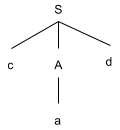
\includegraphics[width=0.3\textwidth]{ParseTree.png}
\caption{Parse Tree for string cad}
\label{fig:Parse Tree}
\end{figure}

\end{example}

There are several difficulties with this parsing technique. One of them is Left-recursion. A grammar G is said to be left-recursive if it has a non-terminal A such that there is a derivation $A\overset{+}{\Rightarrow}A\alpha$ ($\overset{+}{\Rightarrow}$ represents derivation in 1 or more steps) for some $\alpha$. A left-recursive grammar can cause the top-down parser to go into an infinite loop. Hence such grammars are not LL(1) and are not supported by LL Parsing.

Another issue with this parsing technique is left-factoring. Suppose if we have a production such as: A $\to$ abc | ab, then on seeing a, we could not tell, which production to choose, in order to expand the statement. For solving this problem, left-factoring is performed on the grammar. It is the process of factoring out the common prefixes of alternates. The following example explains the procedure of left-factoring:
\begin{example}
If A$\to$ $\alpha\beta$ | $\alpha\gamma$ are two productions in the grammar, then after left-factoring, the production rules are of the form:

A $\to$ $\alpha A'$

A' $\to$ $\beta$ | $\gamma$
\end{example}
To parse an input string using LL parsing, LL Parsing table is required. Following is a brief description of a LL parsing table and the calculation of LL parsing moves.

\paragraph{LL Parsing Table}\mbox{}\\
\label{para: LL Paring Table}
It is a two-dimensional array M[A, b], where A is a non-terminal and b is a terminal or \$. The entries in the LL parsing table are filled by using FIRST and FOLLOW sets. An input string is parsed by using this table.

Algorithm \ref{algo:LL Parsing Table} described below, can be used to construct the LL parsing table for a grammar G.
\begin{algorithm}
\caption{Construction of LL Parsing Table}
\label{algo:LL Parsing Table}

\begin{algorithmic}[1]
\Require Grammar G.
\Ensure Parsing Table M.
\State For each production A $\to$ $\alpha$ of the grammar, do steps 2 and 3.
\State For each terminal a in FIRST($\alpha$), add A $\to$ $\alpha$ to M[A, a].
\State If $\epsilon$ is in FIRST($\alpha$), add A $\to$ $\alpha$ to M[A, b] for each terminal b in FOLLOW(A). If $\epsilon$ is in FIRST($\alpha$) and \$ is in FOLLOW(A), add A $\to$ $\alpha$ to M[A, \$].
\State Make each undefined entry of M error.
\end{algorithmic}
\end{algorithm}

The undefined entries are usually left blank, instead of writing error in them.
\begin{example}
\label{ex:LL table}
For the grammar used in example \ref{ex:First}, LL Parsing table can be filled using the above algorithm as:
\begin{center}
\begin{tabular}{ |c|c|c|c|c| } 
 \hline
  & \textbf{0} & \textbf{1} & \textbf{+} & \textbf{\$} \\
 \hline
 \textbf{T} & T $\to$ 0 & T $\to$ 1 &  &  \\
 \hline
 \textbf{E} & E $\to$ T E' & E $\to$ T E' &  &  \\
 \hline
 \textbf{E'} &  &  & E' $\to$ + E & E' $\to$ $\epsilon$ \\
 \hline
\end{tabular}
\end{center}
\end{example}
A grammar is said to be LL(1) if there are no multiply-defined entries in its parsing table. Left-recursive grammars are not LL(1). Also, left-factoring must be performed on grammars if required, otherwise, they may result in multiple entries in a cell of LL parsing table.

\paragraph{LL Parsing Moves}\mbox{}\\
\label{para: LL Parsing Moves}
The parser has an input, a stack, a parsing table, and an output as shown in figure \ref{fig:LL Parser}.
\begin{figure}
\centering
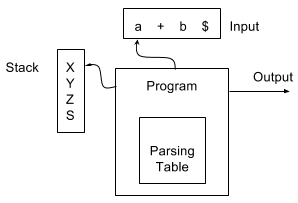
\includegraphics[width=0.5\textwidth]{LLParsingModel.png}
\caption{Model of a predictive parser}
\label{fig:LL Parser}
\end{figure}
The input contains the string to be parsed, followed by \$, the right endmarker. The stack contains a sequence of grammar symbols, preceded by \$ (the bottom-of-stack marker). The contents of the stack, in each step, show the leftmost derivation on the input string. Output shows the action done in each step.

If X is the symbol on top of the stack and a is the current input symbol, then following are the rules that determine the action of the parser.
\begin{enumerate}
\item If X = a = \$, the parser halts and announces successful completion of parsing.
\item If X = a $\neq$ \$, the parser pops X off the stack and advances the input pointer to the next input symbol.
\item If X is a nonterminal, the program consults entry M[X, a] of the parsing table M. If M[X, a] = {X $\to$ UVW}, the parser replaces X on top of the stack by WVU (with U on top). If M[X, a] = error, the parser calls an error recovery routine.
\end{enumerate}

The following example shows the parsing of an input string by applying the above rules. Initially, the stack contains the start symbol of the grammar preceded by \$.
\begin{example}
\label{ex:LL moves}
For the same grammar used in example \ref{ex:First}, if the input string is "0 + 1", then the parsing moves are:
\begin{center}
\begin{tabular}{ |>{\raggedright\arraybackslash$}p{3cm}<{$}|>{\raggedleft\arraybackslash$}p{3cm}<{$}|c| } 
 \hline
 \textbf{STACK} & \textbf{INPUT} & \textbf{OUTPUT} \\
 \hline
 \$ E & 0 + 1 \$ & \\
 \$ E' T & 0 + 1 \$ & E $\to$ T E' \\ 
 \$ E' 0 & 0 + 1 \$ & T $\to$ 0 \\
 \$ E' & + 1 \$ & \\
 \$ E + & + 1 \$ & E' $\to$ + E \\
 \$ E & 1 \$ & \\  
 \$ E' T & 1 \$ & E $\to$ T E' \\
 \$ E' 1 & 1 \$ & T $\to$ 1 \\
 \$ E' & \$ & \\
 \$ & \$ & E' $\to \epsilon$ \\
 \hline
\end{tabular}
\end{center}
\end{example}

\subsubsection{SLR Parsing}
\label{ssubsec:SLR Parsing}
It is one of the LR parsing techniques. It is a bottom-up parsing method. As the name implies, LR parsers scan the input from left-to-right and construct a rightmost derivation in reverse. SLR stands for Simple LR Parsing. K is usually 1 for this parsing. It is the easiest to implement, but may fail to produce a table for certain grammars.

This parsing works on left-recursive grammars, but it is necessary to perform left-factoring if required.

To construct the SLR parsing table, the canonical collection of SLR items are calculated. In later parts of this section, a brief discussion about canonical sets, SLR parsing table and moves is given.

\paragraph{Canonical Collection of SLR Items}\mbox{}\\
\label{para:Canonical Set}
To construct the parsing table, a DFA from the grammar is constructed. The DFA recognizes viable prefixes of the grammar, that is, prefixes of right-sentential forms that do not contain any symbols to the right of the handle.

SLR item of a grammar G is defined as a production of G with a dot at some position on the right side, which indicates how much of a production we have seen at a given point in the parsing process. Thus, production $A\rightarrow XYZ$ generates the four items:

$A\rightarrow .XYZ$

$A\rightarrow X.YZ$

$A\rightarrow XY.Z$

$A\rightarrow XYZ.$

and the production "$A\rightarrow \epsilon$" generates only one item, "$A\rightarrow.$" . As an example, the second item in the above productions, would indicate that we have just seen on the input, a string derivable from X and that we next expect to see a string derivable from YZ. These items are grouped together as itemsets, which are further grouped to form a Canonical SLR collection. To construct this collection we need to define an augmented grammar and two functions - CLOSURE and GOTO.

\begin{itemize}
\item \textbf{Augmented Grammar:} If G is a grammar with start symbol S, then G', the augmented grammar for G, is G with a new start symbol S' and production $S'\rightarrow S$. This new starting production is used to indicate to the parser when it should stop parsing and announce acceptance of the input. This would occur when the parser was about to reduce by $S'\rightarrow S$.

\item \textbf{CLOSURE:} If I is a set of items for a grammar G, then the set of items CLOSURE(I) is constructed from I by the rules:
\begin{enumerate}
\item Every item in I is in CLOSURE(I).
\item If $A\rightarrow\alpha.B\beta$ is in CLOSURE(I) and $B\rightarrow\gamma$ is a production, then add the item $B\rightarrow.\gamma$ to I, if it is not already there.
\end{enumerate}

Following example illustrate the CLOSURE function:
\begin{example}
\label{ex:Closure}
Suppose the augmented grammar is:

$E''\rightarrow E$

$E\rightarrow TE'$

$E'\rightarrow \epsilon | +E$

$T\rightarrow 0 | 1$

If I is the set of one item {[$E''\rightarrow .E$]}, then CLOSURE(I) contains the items

E'' $\rightarrow$ .E

E $\rightarrow$ .TE'

T $\rightarrow$ .1

T $\rightarrow$ .0
\end{example}

\item \textbf{GOTO:} GOTO(I, X), where I is a set of items and X is a grammar symbol, is the closure of the set of all items $[A\rightarrow\alpha X.\beta]$ such that $[A\rightarrow\alpha.X\beta]$ is in I.
Following example illustrates the calculation of GOTO function:
\begin{example}
For the augmented grammar used in example \ref{ex:Closure}, if I is the set of items \{$[E''\rightarrow.E]$, $[E\rightarrow .TE']$, $[T\rightarrow.0]$, $[T\rightarrow.1]$\}, then GOTO(I, T) consists of:

E $\to$ T.E'

E' $\to$ .
    
E' $\to$ .+E
\end{example}
\end{itemize}

The algorithm \ref{algo:SLR Canonical Set} is used to construct C, the canonical collection of sets of LR(0) items for an augmented grammar G'.
\begin{algorithm}
\caption{Canonical collection of sets of SLR items Construction}
\label{algo:SLR Canonical Set}

\begin{algorithmic}[1]
\State C = {CLOSURE(${S'\rightarrow.S}$)}
\Repeat
\For{each set of items I in C and each grammar symbol X such that GOTO(I, X) is not empty and is not in C}
\State add GOTO(I, X) to C
\EndFor
\Until{no more sets of items can be added to C}
\end{algorithmic}
\end{algorithm}

Following example illustrates the construction of collection of sets of LR(0) items:

\begin{example}
\label{ex:SLR set}
For the augmented grammar used in example \ref{ex:Closure}, SLR Canonical set is
\begin{itemize}
\item[I0:] T $\to$ .1 \\
           T $\to$ .0 \\
           E'' $\to$ .E \\
           E $\to$ .TE'
\item[I1:] E $\to$ T.E' \\
           E' $\to$ . \\
           E' $\to$ .+E
\item[I2:] T $\to$ 1.
\item[I3:] T $\to$ 0.
\item[I4:] E'' $\to$ E.
\item[I5:] T $\to$ .1 \\
           E $\to$ .TE' \\
           E' $\to$ +.E \\
           T $\to$ .0
\item[I6:] E $\to$ TE'.
\item[I7:] E' $\to$ +E.
\end{itemize}
\end{example}

\paragraph{SLR Parsing Table}\mbox{}\\
\label{para:SLR Parsing Table}
This table is divided into two parts - Action and Goto. Algorithm \ref{algo:SLR Parsing Table} shows the construction of 
SLR parsing action and goto functions from the DFA that recognizes viable prefixes. Each entry in the table determines whether to shift the input symbol on the stack or to reduce a string of symbols on top of stack by a single symbol using the productions of grammar.

\begin{algorithm}
\caption{Construction of SLR Parsing Table}
\label{algo:SLR Parsing Table}

\begin{algorithmic}[1]
\Require C, the canonical collection of sets of items for an augmented grammar G'.
\Ensure If possible, an LR parsing table consisting of a parsing action function ACTION and a goto function GOTO.
\Statex Let C = {I_0, I_1,...., I_n}. The states of the parser are 0, 1,..., n, state i being constructed from I_i. The parsing actions for state i are determined as follows:
\If{$[A\rightarrow\alpha.a\beta]$ is in I_i and GOTO(I_i, a) = I_j} \label{line:shift}
\State set ACTION[i, a] to "shift j". Here a is a terminal.
\EndIf
\If{$[A\rightarrow\alpha.]$ is in I_i}
\State set ACTION[i, a] to "reduce $A\rightarrow\alpha$" for all a in FOLLOW(A).
\EndIf
\If{$[S'\rightarrow\alpha S.]$ is in I_i}
\State set ACTION[i, \$] to "accept".
\EndIf
\Statex The goto transitions for state i are constructed using the rule:
\If{GOTO(I_i, A) = I_j}
\State GOTO[i, A] = j.
\EndIf  \label{line:goto}
\State All entries not defined by rules \ref{line:shift} through \ref{line:goto} are made "error".
\State The initial state of the parser is the one constructed from the set of items containing [S'$\rightarrow$ .S].
\end{algorithmic}
\end{algorithm}

Following example shows the SLR parsing table for an augmented grammar.
\begin{example}
\label{ex:SLR table}
For the grammar used in example \ref{ex:Closure}, SLR Parsing table is
\begin{center}
\begin{tabular}{ |c|c|c|c|c|c|c|c| }
 \hline
 \textbf{STATE} & \multicolumn{4}{c}{\textbf{ACTION}} & \multicolumn{3}{|c|}{\textbf{GOTO}}\\
 \hline
  & \textbf{0} & \textbf{1} & \textbf{+} & \textbf{\$} & \textbf{T} & \textbf{E} & \textbf{E'}\\
 \hline
 \textbf{0} & s3 & s2 &  &  & 1 & 4 & \\
 \hline
 \textbf{1} &  &  & s5 & r4 &  &  & 6\\
 \hline
 \textbf{3} &  &  & r1 & r1 &  &  & \\
 \hline
 \textbf{4} &  &  &  & accept &  &  & \\
 \hline
 \textbf{5} & s3 & s2 &  &  & 1 & 7 & \\
 \hline
 \textbf{6} &  &  &  & r3 &  &  & \\
 \hline
 \textbf{7} &  &  &  & r5 &  &  & \\
 \hline
\end{tabular}
\end{center}
Blank entries are the "error" entries.
\end{example}

\paragraph{SLR Parsing Moves}\mbox{}\\
\label{para: SLR Parsing Moves}
An LR parser consists of two parts - a driver routine and a parsing table. The driver routine is the same for all LR parsers, but the parsing table changes from one parser to another. Figure \ref{fig:LR Parser} shows the model of LR Parsers.
\begin{figure}
\centering
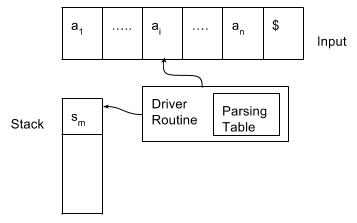
\includegraphics[width=0.5\textwidth]{SLRParsingModel.png}
\caption{Model of a SLR parser}
\label{fig:LR Parser}
\end{figure}

The input is read from left to right, one symbol at a time. The stack contains a string of the form s_0X_1s_1X_2s_2....X_ms_m, where s_m is on top. Each X_i is a grammar symbol and each s_i is the state.

The entry ACTION[s_m, a_i], where s_m is the state on top of stack and a_i is the current input symbol, can have one of four values:
\begin{enumerate}
\item shift s.
\item reduce $A\rightarrow\beta$.
\item accept.
\item error.
\end{enumerate}
The function GOTO takes a state and grammar symbol as arguments and produces a state.

A configuration of an LR parser is a pair whose first component is the stack contents and whose second component is the unexpected input:

(s_0 X_1 s_1 X_2 s_2 ... X_m s_m, a_i a_{i+1} ... a_n \$)

The configurations resulting after each of the four types of move, on consulting the parsing action table entry ACTION[s_m, a_i], are as follows:
\begin{enumerate}
\item If ACTION[s_m, a_i] = shift s, the parser executes a shift move, entering the configuration

(s_0 X_1 s_1 X_2 s_2 ... X_m s_m a_i s, a_{i+1} ... a_n \$)

Here the parser has shifted the current input symbol a_i and the next state s = GOTO[s_m, a_i] onto the stack. a_{i+1} becomes the new current input symbol.
\item If ACTION[s_m, a_i] = reduce $A\rightarrow\beta$, then the parser executes a reduce move, entering the configuration

(s_0 X_1 s_1 X_2 s_2 ... X_{m-r} s_{m-r} A s, a_i a_{i+1} ... a_n \$)

where s = GOTO[s_{m-r}, A] and r is the length of $\beta$, the right side of the production. Here the parser first popped 2r symbols off the stack (r state symbols and r grammar symbols), exposing state s_{m-r}. The parser then pushed both A, the left side of the production, and s, the entry for ACTION[s_{m-r}, A], onto the stack. The current input symbol is not changed in a reduce move. For the LR parsers we shall construct, X_{m-r+1} ... X_m, the sequence of grammar symbols popped off the stack, will always match $\beta$, the right side of the reducing production.
\item If ACTION[s_m, a_i] = accept, parsing is completed.
\item If ACTION[s_m, a_i] = error, the parser has discovered an error and calls an error recovery routine.
\end{enumerate}

Following example illustrates the calculation of LR Parsing moves:
\begin{example}
\label{ex:SLR Moves}
For the augmented grammar used in example \ref{ex:Closure}, if the input string is 0 + 1, then paring moves are:
\begin{center}
\begin{tabular}{ |>{\raggedright\arraybackslash$}p{3.5cm}<{$}|>{\raggedleft\arraybackslash$}p{3.5cm}<{$}|}
 \hline
 \textbf{STACK} & \textbf{INPUT} \\
 \hline
 0 & 0 + 1 \$ \\
 0 0 3 & + 1 \$ \\
 0 T 1 & + 1 \$ \\
 0 T 1 + 5 & 1 \$ \\
 0 T 1 + 5 1 2 & \$ \\
 0 T 1 + 5 T 1 & \$ \\
 0 T 1 + 5 T 1 E' 6 & \$ \\
 0 T 1 + 5 E 7 & \$ \\
 0 T 1 E' 6 & \$ \\
 0 E 4 & \$ \\
 \hline
\end{tabular}
\end{center}
\end{example}

\chapter{Overview of the Tool}
\label{chap:overview}
This chapter gives an overview of the tool. It describes the tool from a high level of abstraction in order to give a basic understanding of how it works. There are two main components of the tool - the Core Engine and Interface.

\section{Core Engine}
\label{sec:core engine}
There are 5 phases of program compilation - lexical analysis, syntax analysis (parsing), semantic analysis, code optimization and code generation, as described in chapter \ref{chap:background}. This tool is developed for the parsing phase of compiler. Questions are generated to teach various parsing techniques in compiler. These questions are of the form of Multiple Choice Questions (MCQ). The questions are of two types - primary questions and hint questions. The primary questions are of the form of Multiple Choice Multiple Answers (MCMA), while the hint questions are of the form of Multiple Choice Single Answers (MCSA). The system takes a grammar as input and uses that to generate questions in the subsequent stages. Figure 2.1 shows the work-flow of the tool. The different steps in the work-flow are describe below:
\begin{figure}
\centering
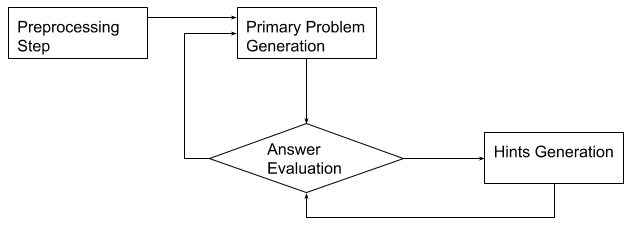
\includegraphics[width=1\textwidth]{CoreEngine.png}
\caption{Core Engine}
\label{fig:core engine}
\end{figure}

\subsection{Preprocessing}
\label{subsec:preprocessing}
The system takes a grammar as input and performs the necessary processing required to generate problems on and evaluate the solution given by the student, for these problems. Processing includes determining FIRST set, FOLLOW set, LL Parsing Table, LL Parsing moves (on the input string given by the user), SLR Canonical Set of items, SLR Parsing Table and SLR Parsing Moves (on the input string given by the user). These are calculated using the rules described in chapter \ref{chap:background}.

The preprocessing performed depends on the domain of questions to be generated. This option is given by the user. The data structures generated in the preprocessing step are used as input in the next stages of problem generation.

\subsection{Primary Problem Generation}
\label{subsec:primary problem generation}
Based on the choice of technique made by the user, primary problems are generated for that domain. For each technique, certain data structures are generated as described in section \ref{subsec:preprocessing}. The tool generates questions on the basis of these data structures. All possible values of these data structures are given as options for the MCQs. Users have to select multiple options which collectively form the solution to the problem.

\begin{example}
\label{ex:Primary Prob Gen}
For the grammar used in example \ref{ex:First}, if a user makes a choice of FIRST set, to generate questions, then questions will be generated for all the non-terminals in the grammar. They are of the form:

Which symbols should be included in FIRST[sym] (where sym represents the non-terminals in the grammar) ?

\textbf{Options:} terminals in the grammar

For this grammar, non-terminals are E', E and T, and the terminals are 1, 0 and +.
\end{example}

This type of primary question is used for all the techniques. But variations occur for some of the techniques. For example, in the case of GOTO function in SLR Canonical set, there are two types of primary questions:
\begin{example}
\label{ex:goto primary problems}
Suppose the grammar used in example \ref{ex:First}, then one type of primary question is

If I is the set of items { [E $\to$ T.E'], [E' $\to$ .], [E' $\to$ .+E], } and X is the symbol +, then which of the following items will be contained in GOTO(I, X) ?

\textbf{Options:} E' $\to$ +.E \quad T $\to$ .0 \quad T $\to$ .1 \quad T $\to$ 1. \quad E $\to$ .TE' \quad T $\to$ 0. \quad E'' $\to$ .E \quad E'' $\to$ E.

And the other type is

In GOTO(I, X), if X is the grammar symbol E, then which of the following itemsets can act as I to get itemset {[E' $\to$ +E.]} as result ?

\textbf{Options:}

I0: T $\to$ .1 \quad E'' $\to$ .E \quad T $\to$ .0 \quad E $\to$ .TE'

I1: E $\to$ T.E' \quad E' $\to$ . \quad E' -> .+E

I2: T $\to$ 1.

I3: T $\to$ 0.

I4: E'' $\to$ E.

I5: T $\to$ .0 \quad E $\to$ .TE' \quad E' $\to$ +.E \quad T $\to$ .1

I6: E $\to$ TE'.    

I7: E' $\to$ +E.
\end{example}

In some cases, problems are generated for all the values in the data structure generated in the preprocessing step. But in most other cases, the tool selects a random subset of these values. Then the system generates problems on these values. For example, if the questions are to be generated for LL Parsing Table, then instead of filling entries in all the cells of parsing table, random indexes of the cells of LL Parsing table are chosen and the tool generates questions only for those cells.
\begin{example}
\label{ex:random number}
Which grammar rules should be included in the highlighted cell of the LL parsing table ?

\textbf{Options:} T $\to$ 0 \quad T $\to$ 1 \quad E $\to$ T E' \quad E' $\to$ $\epsilon$ \quad E' $\to$ + E \quad ERROR
\begin{center}
\begin{tabular}{ |c|c|c|c|c| } 
 \hline
  & \textbf{0} & \textbf{1} & \textbf{+} & \textbf{\$} \\
 \hline
 \textbf{T} &   &   & ERROR & ERROR \\
 \hline
 \textbf{E} & E $\to$ T E' &   & ERROR & ERROR \\
 \hline
 \textbf{E'} & ERROR & ERROR & E'$\to$ + E & ? \\
 \hline
\end{tabular}
\end{center}

Which grammar rules should be included in the highlighted cell of the LL parsing table ?

\textbf{Options:} T $\to$ 0 \quad T $\to$ 1 \quad E $\to$ T E' \quad E' $\to$ $\epsilon$ \quad E' $\to$ + E \quad ERROR
\begin{center}
\begin{tabular}{ |c|c|c|c|c| } 
 \hline
  & \textbf{0} & \textbf{1} & \textbf{+} & \textbf{\$} \\
 \hline
 \textbf{T} &   &   & ERROR & ERROR \\
 \hline
 \textbf{E} & E $\to$ T E' & ? & ERROR & ERROR \\
 \hline
 \textbf{E'} & ERROR & ERROR & E'$\to$ + E &  \\
 \hline
\end{tabular}
\end{center}

Which grammar rules should be included in the highlighted cell of the LL parsing table ?

\textbf{Options:} T $\to$ 0 \quad T $\to$ 1 \quad E $\to$ T E' \quad E' $\to$ $\epsilon$ \quad E' $\to$ + E \quad ERROR
\begin{center}
\begin{tabular}{ |c|c|c|c|c| } 
 \hline
  & \textbf{0} & \textbf{1} & \textbf{+} & \textbf{\$} \\
 \hline
 \textbf{T} & ? &   & ERROR & ERROR \\
 \hline
 \textbf{E} & E $\to$ T E' &   & ERROR & ERROR \\
 \hline
 \textbf{E'} & ERROR & ERROR & E'$\to$ + E &  \\
 \hline
\end{tabular}
\end{center}

Which grammar rules should be included in the highlighted cell of the LL parsing table ?

\textbf{Options:} T $\to$ 0 \quad T $\to$ 1 \quad E $\to$ T E' \quad E' $\to$ $\epsilon$ \quad E' $\to$ + E \quad ERROR
\begin{center}
\begin{tabular}{ |c|c|c|c|c| } 
 \hline
  & \textbf{0} & \textbf{1} & \textbf{+} & \textbf{\$} \\
 \hline
 \textbf{T} &   & ? & ERROR & ERROR \\
 \hline
 \textbf{E} & E $\to$ T E' &   & ERROR & ERROR \\
 \hline
 \textbf{E'} & ERROR & ERROR & E'$\to$ + E &  \\
 \hline
\end{tabular}
\end{center}

\end{example}

\subsection{Answer Evaluation}
\label{subsec:answer evaluation}
In this step, the solution given by the user for the problem generated in the previous step, is evaluated. In order to achieve this, the solution given by the user is compared with the data structure computed by the tool in the preprocessing step. If both the solutions match, then the control transfers to the primary Problem Generation step again, as described in section \ref{subsec:primary problem generation}, where it generates the question for the next value.

However, if the solution is wrong, the tool finds the degree of correctness of the solution provided by the user. This implies that the tool takes into account, the incorrect options which are marked in the solution as well as the options in the correct solution which are not marked by the user as a part of her solution. For all such options, hint questions are generated in the next step, in order to guide the user to the correct solution of the problem generated in the previous step.
\begin{example}
\label{ex:answer evaluation}
Suppose that the primary question generated is:

Which symbols should be included in FIRST[T] ?

\textbf{Options:} 1 \qquad 0 \qquad +

Now consider that the user gives the solution as {+ , 0}, whereas the right solution is {0, 1}. On comparison, the system finds that the solution given by the user is wrong. The system thus classifies '+' as incorrectly chosen option and '1' as correct option omitted by the user.
\end{example}

\subsection{Hints Generation}
\label{subsec:hints generation}
In this step, the system generates hint questions when the solution provided by the user is incorrect. Questions are generated, taking into account, the incorrect options marked by the user, as well as the correct options omitted by the user, in her provided solution.

There are two types of hint questions which are generated for all the parsing techniques:
\begin{itemize}
\item \textbf{H1:} This type of question is generated for the incorrect options marked in the solution, in order to give a hint to the user that the option marked is wrong.
\item \textbf{H2:} This is the other type of question which is generated for the correct options which are omitted by the user. The tool generates a MCSA question which tries to make the user realize the sort of scenarios in which the omitted option should be chosen.
\end{itemize}

Below is a detailed explanation of these questions:
\begin{itemize}
\item \textbf{H1:}
These types of questions are generated in both cases when a correct option is omitted as well as when an incorrect option is chosen. It helps the user understand the rules used in the technique, by which a particular option must or must not be a part of the solution.
\begin{example}
\label{ex:ques type 1}
For the grammar used in example \ref{ex:First}, if the primary question is generated for FIRST[T] and the choices marked by the user are {1, +}, then as '+', is an incorrect option, the hint question of type 1 is generated as:

According to which of the following rules, '+' is a part of FIRST[T] ?  
\begin{enumerate}
\item If X is a terminal, then FIRST(X) is \{X\}.
\item If X is a non-terminal and X $\to$ a$\alpha$ is a production, then add a to FIRST(X). If X $\to$ $\epsilon$ is a production, then add $\epsilon$ to FIRST(X).
\item If $X \to\ Y_1Y_2....Y_k$ is a production, then for all i such that all of $Y_1,....,Y_{i-1}$ are non-terminals and FIRST($Y_j$) contains $\epsilon$ for $j = 1, 2, ...., i-1$ (i.e $Y_1Y_2....Y_{i-1} \to \epsilon$), add every non-$\epsilon$ symbol in FIRST($Y_i$) to FIRST($X$). If $\epsilon$ is in FIRST($Y_j$) for all j = 1, 2, ....., k, then add $\epsilon$ to FIRST(X).
\item No valid rule for this symbol.
\end{enumerate}
\end{example}
\textbf{Options:} $1 \qquad 2 \qquad 3 \qquad 4$

\item \textbf{H2:}
This question is only generated if correct options in the solution are omitted by the user. It helps the user to realize that the omitted option must be a part of the correct solution.
\begin{example}
\label{ex:ques type 2}
For the correct option '0' left out by the user in example \ref{ex:ques type 1}, hint question of type 2 is generated as:

Should '0' be included in FIRST[T] ?

\textbf{Options:} Yes $\qquad$ No
\end{example}
\end{itemize}

Then question of type 1 (H1) is also generated for '0' by the system. This helps the user to understand the rules of the techniques properly. Thus, these questions direct the student to the correct solution of the primary question.

For the special case of LL Parsing Table, we have also introduced another type of hint question (H3). A parsing table is a data structure which is used to parse input strings using the grammar. Previously, these input strings were taken as input, as there was no defined way through which the tool can generate one. The current tool, generates these input strings automatically.

If any cell of the parsing table is filled incorrectly, then there exists a valid string for that cell, which is accepted by the grammar, but can not be parsed correctly by the newly filled parsing table. So the system is designed in such a way that it generates the smallest possible input string for the incorrectly filled cell of the LL Parsing Table. Then the hint question is generated using this string, in which the user is presented with the parsing moves on this input string, using the LL Parsing table filled by the user. This gives her a hint that the incorrect entry is filled in that cell.

\begin{example}
\label{ex:LL table input string question}
For the grammar used in example \ref{ex:First}, if the primary question is asked to fill the cell M[E'][+] of the LL Parsing Table M. And the entry filled is E' $\to$ $\epsilon$, then the system will generate hint question as:

\begin{center}
\begin{tabular}{ |c|c|c| } 
 \hline
 \textbf{STACK} & \textbf{INPUT} & \textbf{OUTPUT} \\
 \hline
 \$ E & 0 + 1 \$ & \\
 \$ E' T & 0 + 1 \$ & E $\to$ T E' \\ 
 \$ E' 0 & 0 + 1 \$ & T -> 0 \\
 \$ E' & + 1 \$ & \\ 
 \$ & + 1 \$ & E' $\to$ $\epsilon$ \\
 \hline
\end{tabular}
\end{center}

\begin{center}
\begin{tabular}{ |c|c|c|c|c| } 
 \hline
  & \textbf{0} & \textbf{1} & \textbf{+} & \textbf{\$} \\
 \hline
 \textbf{T} &   &   & ERROR & ERROR \\
 \hline
 \textbf{E} & E $\to$ T E' &   & ERROR & ERROR \\
 \hline
 \textbf{E'} & ERROR & ERROR & E' $\to$ $\epsilon$ & \\
 \hline
\end{tabular}
\end{center}

LL Parsing on this input string is not working correctly due to the wrong entry made in the cell M[E'][+]. Please correct the value in this cell.
%Remove either table or cell name

\textbf{OPTIONS:} T $\to$ 0 \quad T $\to$ 1 \quad E $\to$ T E' \quad E' $\to$ epsilon \quad E' $\to$ + E \quad ERROR  
\end{example}

\chapter{Algorithms}
\label{chap:algorithms}
This chapter gives a description of the work-flow in problem generation and also detailed explanations of the algorithms used to generate problems for the tool. Primary problems along with hint questions are generated for the following broad domains:
\begin{itemize}
\item First and Follow
\item LL Parsing
\item SLR Parsing
\end{itemize}
The LL and SLR parsing problem domains have further sub-domains on which problems are generated by the tool. This chapter covers the algorithms for these sub-domains of problems, along with hint question generation algorithms and a few other auxiliary algorithms.
Problems in the LL Parsing domain involve the following categories:
\begin{itemize}
\item LL parsing table
\item LL parsing moves
\end{itemize}
Problems in the SLR Parsing domain involve the following categories:
\begin{itemize}
\item SLR canonical set
\item SLR parsing table
\item SLR parsing moves
\end{itemize}

The problem generation algorithms make a few assumptions on the grammar given as input. The following are the pre-conditions:
\begin{itemize}
\item Only Context Free Grammar (CFG) must be used.
\item If LL Parsing technique is to be used, then the grammar must not be left-recursive.
\item If the questions are to be generated for Parsing Moves of any Parsing Technique, then it is required that the grammar be unambiguous.
\end{itemize}

\section{Problem Generation Workflow}
\label{sec:Problem Generation}
This section describes the workflow of problem generation. Problems are generated for a specific domain which is chosen by the user. This information, along with the input grammar defines a set of possible problems which can be generated. These problems are known as primary problems. Each of these candidate problems are generated and given to the user to solve. Upon successfully solving one problem, the next candidate problem is presented to the user. The process of learning occurs when the user is not able to solve the presented primary problem. Hint questions are then generated to guide the user into reaching the correct solution and understanding her mistakes. The hint questions are of two types, based on the context on which they are generated:
\begin{itemize}
\item \textbf{H1:} This type of hint question is generated when an incorrect choice is marked by the user in her solution to the primary problem. The question tries to make the user realize that the choice marked is incorrect and should not be a part of the solution.
\item \textbf{H2:} This type of hint question is generated when a correct choice is omitted by the user in the solution set of choices. The generated question tries the help the user understand why the choice should be a part of the solution.
\end{itemize}

The workflow of problem generation is depicted below using several algorithms as depicted below. These algorithms depict the common structure of all algorithms across the various domains. However the exact algorithms for preprocessing, problem generation and hint generation are domain specific, and are elaborated in the subsequent sections.

\begin{algorithm}
\caption{Preprocess grammar to create required data structures}
\label{algo:preprocess}
\begin{algorithmic}[1]
\Function{preprocess}{$D$}
\State S := data structure on the basis of which questions will be generated.
\State A := auxiliary data structures required to compute S and display helpers to users.
\State \Return (S,A)
\EndFunction
\end{algorithmic}
\end{algorithm}

\begin{algorithm}
\caption{Generate questions for a specific domain}
\label{algo:generatequestions}
\begin{algorithmic}[1]
\Function{generate\textunderscore questions}{$D$}
\State (S,A) := \Call{preprocess}{$D$}
\ForAll{context in S}
\State P := \Call{generate\textunderscore primary\textunderscore question}{$context, D$}
\State $answered \gets false$
\While{$answered = false$}
\State $answered \gets \Call{evaluate\textunderscore primary\textunderscore question}{P, D}$
\EndWhile
\EndFor
\EndFunction
\end{algorithmic}
\end{algorithm}

\begin{algorithm}
\caption{Generate primary question based on a context in a specific domain}
\label{algo:generateprimary}
\begin{algorithmic}[1]
\Function{generate\textunderscore primary\textunderscore question}{$context, D$}
\State P := generated primary question based on D and context
\State \Return P
\EndFunction
\end{algorithmic}
\end{algorithm}

\begin{algorithm}
\caption{Evaluate primary question generated previously}
\label{algo:evaluateprimary}
\begin{algorithmic}[1]
\Require C = \{c | c $\in$ correct(P)\}
\Require I = \{c | c $\in$ incorrect(P)\}
\Function{evaluate\textunderscore primary}{$P, D$}
\State Display P to user
\State CHOICES := read set of choices from user
\If{$ CHOICES = C$}
\State Display "correct solution"
\State \Return true
\Else
\ForAll{choice in CHOICES}
\If{choice$\in$ I}
\State $H1 \gets \Call{generate\textunderscore hint\textunderscore question}{choice, P, D, 1}$
\State \Call{evaluate\textunderscore hint\textunderscore question}{$H1$}
\ElsIf{choice$\in$ C}
\State $C \gets C - \{choice\}$
\EndIf
\EndFor
\If{C$\neq \emptyset$}
\ForAll{choice $\in$ C}
\State $H2 \gets \Call{generate\textunderscore hint\textunderscore question}{choice, P, D, 2}$
\State \Call{evaluate\textunderscore hint\textunderscore question}{$H2$}
\State $H1 \gets \Call{generate\textunderscore hint\textunderscore question}{choice, P, D, 1}$
\State \Call{evaluate\textunderscore hint\textunderscore question}{$H1$}
\EndFor
\EndIf
\State \Return false
\EndIf
\EndFunction
\end{algorithmic}
\end{algorithm}

\begin{algorithm}
\caption{Generate hint question based on choice, problem and domain}
\label{algo:generatehint}
\begin{algorithmic}[1]
\Function{generate\textunderscore hint\textunderscore question}{$choice, P, D, type$}
\State H := generated hint question based on type, options of P, choice and domain D
\State \Return H
\EndFunction
\end{algorithmic}
\end{algorithm}

\begin{algorithm}
\caption{Evaluate hint question generated previously}
\label{algo:evaluatehint}
\begin{algorithmic}[1]
\Require C := correct choice for H
\Function{evaluate\textunderscore hint\textunderscore question}{$H$}
\State $correct \gets false$
\While{$\neg correct$}
\State display H
\State read choice
\If{choice = C}
\State correct = true
\Else
\State correct = false
\EndIf
\EndWhile
\State display "correct solution"
\EndFunction
\end{algorithmic}
\end{algorithm}

\section{First and Follow}
\label{sec:firstandfollow}
This domain of the problems attempts to teach First and Follow sets in compilers. The procedures that are specific to this domain include preprocessing, primary problem generation and hint question generation. We shall describe each of these procedures below.

\subsection{First}
\label{subsec:ff-first}

Preprocessing for generation of questions in the First domain involves computation of first sets for all non-terminals in the grammar. This is depicted in algorithm \ref{algo:preprocess-first}. Algorithm \ref{algo:primary-first} shows how primary problems are generated for a specific context derived from the preprocessing stage. Further, algorithm \ref{algo:hint-first} explains the procedure for generating hint questions of a specified type and based on a choice from the solution set.

\begin{algorithm}
\caption{Preprocessing for First}
\label{algo:preprocess-first}
\begin{algorithmic}[1]
\Function{preprocess\textunderscore first}{$G$}
\State N := set of all non-terminals in grammar G
\State S := table for storing all first sets
\ForAll{n in N}
\State F := \{ t | t$\in$ first(n)\}
\State S[n] = F
\EndFor
\State \Return S
\EndFunction
\end{algorithmic}
\end{algorithm}

\begin{algorithm}
\caption{Primary problem generation for First}
\label{algo:primary-first}
\begin{algorithmic}[1]
\Function{generate\textunderscore primary\textunderscore question\textunderscore first}{$context, S$}
\State Q := "Which symbols should be included in FIRST[context] ?"
\State F = S[context]
\State \Return (Q, F)
\EndFunction
\end{algorithmic}
\end{algorithm}

In algorithm \ref{algo:hint-first}, hint question H (H1) contains all the rules described in \ref{ssubsec:preliminary}, required to generate first set for each symbol in the grammar. Answer to this hint question contains the rule number which is satisfied by the choice.
\begin{algorithm}
\caption{Hint question generation for First}
\label{algo:hint-first}
\begin{algorithmic}[1]
\Function{generate\textunderscore hint\textunderscore question\textunderscore first}{$choice, P, D, type, context$}
\If{type = 1}
\State H := "According to which of the rules of first, choice is a part of FIRST[context] ? 1. If X is a terminal, ..... 4. No valid rule for this symbol."
\If{choice$\in$ I}
\State A := 4
\ElsIf{choice$\in$ C}
\State A := 1 or 2 or 3
\EndIf
\ElsIf{type = 2}
\State H := "Should choice be included in FIRST[context] ?"
\State A := "Yes"
\EndIf
\State \Return (H, A)
\EndFunction
\end{algorithmic}
\end{algorithm}

\subsection{Follow}
\label{subsec:ff-follow}

Preprocessing for generation of problems in the Follow domain, involves computing First and Follow sets for the given grammar. This is shown in algorithm \ref{algo:preprocess-follow}. The procedures for primary problem generation and hint question generation are shown in algorithms \ref{algo:primary-follow} and \ref{algo:hint-follow} respectively.

\begin{algorithm}
\caption{Preprocessing for Follow}
\label{algo:preprocess-follow}
\begin{algorithmic}[1]
\Function{preprocess\textunderscore follow}{$G$}
\State N := set of all non-terminals in grammar G
\State S := table for storing all follow sets
\ForAll{n in N}
\State F := \{ t | t$\in$ follow(n)\}
\State S[n] = F
\EndFor
\State \Return S
\EndFunction
\end{algorithmic}
\end{algorithm}

\begin{algorithm}
\caption{Primary question generation for Follow}
\label{algo:primary-follow}
\begin{algorithmic}[1]
\Function{generate\textunderscore primary\textunderscore question\textunderscore follow}{$context$}
\State Q := "Which symbols should be included in FOLLOW[context] ?"
\State F = S[context]
\State \Return (Q, F)
\EndFunction
\end{algorithmic}
\end{algorithm}

In algorithm \ref{algo:hint-follow}, hint question H (H1) contains all the rules described in \ref{ssubsec:preliminary}, required to generate follow set for each symbol in the grammar. Answer to this hint question contains the rule number which is satisfied by the choice.

\begin{algorithm}
\caption{Hint question generation for Follow}
\label{algo:hint-follow}
\begin{algorithmic}[1]
\Function{generate\textunderscore hint\textunderscore question\textunderscore follow}{$choice, type, context$}
\If{type = 1}
\State H := "According to which of the rules of follow, choice is a part of FOLLOW[context] ? 1. \$ is in FOLLOW(S), ..... 4. No valid rule for this symbol."
\If{choice$\in$ I}
\State A := 4
\ElsIf{choice$\in$ C}
\State A := 1 or 2 or 3
\EndIf
\ElsIf{type = 2}
\State H := "Should choice be included in FOLLOW[context] ?"
\State A := "Yes"
\EndIf
\State \Return (H, A)
\EndFunction
\end{algorithmic}
\end{algorithm}

\section{LL Parsing}
\label{llparsing}

This domain of problems attempts to teach users the LL parsing technique in compilers. Similar to the First and Follow domain, the same procedures have different algorithms that are specific to this domain. We shall be describing these procedures below. This domain is further divided into two sub-domains: LL parsing table and LL parsing moves. The following subsections cover these sub-domains. 

\subsection{LL Parsing Table}
\label{subsec:lltable}

This sub-domain of problems attempts to teach users how to build a LL parsing table. Problems in this sub-domain involve filling out entries in the cells of a LL parsing table. The problems in this sub-domain are split into two levels, depending on the approach used for learning. These levels differ in the type of hint questions that are generated. Both these levels involve generation of a primary question, which instructs the user to fill up missing cells in the parsing table. It is when the user makes a wrong attempt, that the levels come into play:
\begin{itemize}
\item \textbf{Level 1:} The hint questions involve generation of a question of type H1, if an incorrect entry is made in one of the cells. If a correct entry is omitted in the cell, a question of type H2 is generated. This is similar to the work-flow of problem generation in the First and Follow domain. 
\item \textbf{Level 2:} In this level, only one category of hint is generated. It is assumed here that the grammar is unambiguous and hence a cell cannot contain more than one entry. Thus, for each incorrect cell entry in the table, a corresponding input string is generated. This is the shortest possible input string for that cell entry. Using the entries filled up by the user in the parsing table, a sequence of parsing moves on the generated input string is displayed to the user as the hint. The user is then asked to correct the erroneous cell entry in the parsing table, using this information.
\end{itemize}

The preprocessing required for question generation on LL parsing table is shown in algorithm \ref{algo:preprocessing-lltable}. Primary problem generation is described using algorithm \ref{algo:primary-lltable}. Hint question for level 1 is depicted in algorithm \ref{algo:hint-lltable}. Input string generation is described in section \ref{ssec:inputgen}.

Instead of filling all the entries of LL parsing table, the user is asked to fill some entries of the table. For this purpose, Algorithm \ref{algo:preprocessing-lltable} uses 4 random numbers. These random numbers are generated on the index of cells of LL parsing table. The algorithm picks those random indexes one by one and generates primary question along with hint questions.

\begin{algorithm}
\caption{Preprocessing for LL parsing table}
\label{algo:preprocessing-lltable}
\begin{algorithmic}[1]
\Function{preprocessing\textunderscore lltable}{$G, First, Follow, T$}
\State N := set of all non-terminals in grammar G
\State L := LL parsing table 
\ForAll{n in N}
\State D := table containing all the cells of the corresponding n
\ForAll{t in T}
\State F := \{ x | x$\in$ cell[n][t]\}
\State D[t] = F
\EndFor
\State L[n] = D
\EndFor
\State R := set containing 4 random numbers
\State S = \{\}
\ForAll{r in R}
\State index := choose random cell index in table
\State E := context corresponding to index
\State S = S $\cup$ E
\EndFor
\State \Return (L, S)
\EndFunction
\end{algorithmic}
\end{algorithm}

\begin{algorithm}
\caption{Primary problem generation for LL parsing table}
\label{algo:primary-lltable}
\begin{algorithmic}[1]
\Function{generate\textunderscore primary\textunderscore question\textunderscore lltable}{$context$}
\State Q := "Which grammar rules should be included in the context cell of the LL parsing table ?"
\State index := choose random cell index in table
\State n := row name of cell referenced by index
\State t := column name of cell referenced by index
\State F = L[n][t]
\State \Return (Q, F)
\EndFunction
\end{algorithmic}
\end{algorithm}

\begin{algorithm}
\caption{Hint question generation for LL parsing table}
\label{algo:hint-lltable}
\begin{algorithmic}[1]
\Function{generate\textunderscore hint\textunderscore question\textunderscore lltable}{$choice, type$}
\If{type = 1}
\State H := "According to which of the rules of ll parsing table, choice belongs to the context cell ? 1. 1. If A $\rightarrow$ $\alpha$ is a production ..... 4. No valid rule."
\If{choice$\in$ I}
\State A := 4
\ElsIf{choice$\in$ C}
\State A := 1 or 2 or 3
\EndIf
\ElsIf{type = 2}
\State H := "Should choice be a part of the context cell ?"
\State A := "Yes"
\EndIf
\State \Return (H, A)
\EndFunction
\end{algorithmic}
\end{algorithm}

\subsubsection{Input String Generation}
\label{ssec:inputgen}

This section describes the procedure for input string generation for problems in the LL parsing domain. Algorithms \ref{algo:inputstr gen} through \ref{algo:graph gen} show this procedure.

The following example (\ref{ex:inputstr}) depicts the working of the procedure:
\begin{example}
\label{ex:inputstr}
Suppose the grammar is \\
E $\to$ T E' \\
E' $\to$ + T E' | $\epsilon$ \\
T $\to$ F T' \\
T' $\to$ * F T' | $\epsilon$ \\
F $\to$ ( E ) | id

The graph generated by the algorithm for this grammar is shown in Figure \ref{fig:Grammar Graph}.
\begin{figure}
\centering
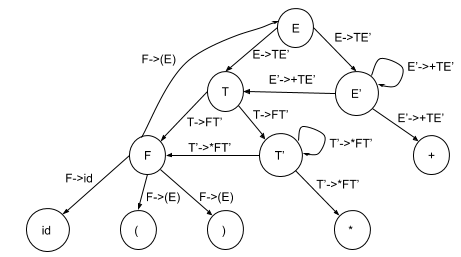
\includegraphics[width=0.8\textwidth]{GrammarGraph.png}
\caption{Graph generated on applying algorithm \ref{algo:graph gen}}
\label{fig:Grammar Graph}
\end{figure}

The node containing the start symbol becomes the source node. Then, we apply Dijkstra's Algorithm to find shortest path from the source to every other node in the graph. The resultant tree is shown in Figure \ref{fig:Dijkstra Tree 1}.
\begin{figure}
\centering
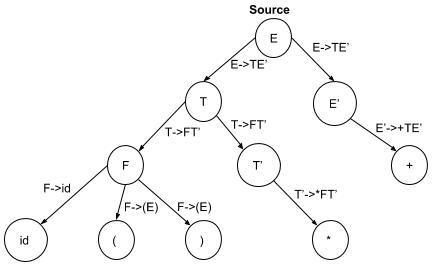
\includegraphics[width=0.8\textwidth]{DijkstraTree1.png}
\caption{Tree after applying Dijkstra Algorithm first time}
\label{fig:Dijkstra Tree 1}
\end{figure}

If the user made an incorrect entry in M[T'][)] of LL Parsing Table (where M refers to the data structure containing the parsing table), then the node corresponding to T' becomes the destination node. The next step in the algorithm is to find the shortest path from the source to the destination in the tree using Dijkstra Algorithm. The path in the tree is shown in Figure \ref{fig:Path 1}.

\begin{figure}
\centering
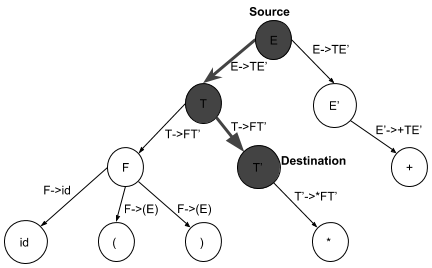
\includegraphics[width=0.8\textwidth]{Path1.png}
\caption{Path in the tree from E to T'}
\label{fig:Path 1}
\end{figure}

Now, in order to build the input string, we have used a stack containing the symbols in the grammar. The stack is just like the stack used for LL Parsing Moves. It consists of all the symbols that occur in the path of input string generation. The stack consists of '\$' initially. All the keys corresponding to the nodes and the symbols on the edges, obtained in the path from source to destination, are pushed on to the stack in the order in which the path is accessed.

If a non-terminal appears on the top of the stack then,
\begin{itemize}
\item if it is the key of a node in the path, the outgoing edge from this node in the path, is pushed on to the stack in reverse order.
\item otherwise the minimum length rule in the grammar for this non-terminal, is pushed on to the stack in reverse order.
\end{itemize}
If a terminal symbol appears on top of the stack, it is popped from the stack and appended to the input string.

Following is the configuration obtained by using the path from E to T' shown in Figure \ref{fig:Path 1}.
\begin{center}
\begin{tabular}{ |c|c| } 
 \hline
 \textbf{stack} & \textbf{input string} \\
 \hline
 \$E & \\
 \$E'T & \\
 \$E'T'F & \\
 \hline
\end{tabular}
\end{center}

On top of the stack, we have symbol F, which is not in the path from E to T', so we replace it by the shortest rule in the grammar for this non-terminal (F $\to$ id). The configuration now becomes
\begin{center}
\begin{tabular}{ |c|c| } 
 \hline
 \textbf{stack} & \textbf{input string} \\
 \hline
 \$E'T'id & \\
 \hline
\end{tabular}
\end{center}

Now, as a terminal appears on top of the stack, it is popped from the stack and becomes a part of the input string. Now the configuration becomes
\begin{center}
\begin{tabular}{ |c|c| } 
 \hline
 \textbf{stack} & \textbf{input string} \\
 \hline
 \$E'T' & id \\
 \hline
\end{tabular}
\end{center}

Now, we have T'(destination) on top of the stack. As there is no rule of T' in the grammar which contains ), we have to find a path from T' to ). For this purpose T' now becomes the source node. Again Dijkstra's algorithm is applied, to find shortest paths from the new source to all other nodes in the graph. Figure \ref{fig:Dijkstra Tree 2} shows the tree obtained after applying Dijkstra algorithm.
\begin{figure}
\centering
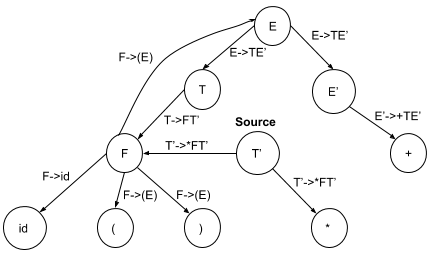
\includegraphics[width=0.8\textwidth]{DijkstraTree2.png}
\caption{Tree after applying Dijkstra Algorithm second time}
\label{fig:Dijkstra Tree 2}
\end{figure}

Now, the node corresponding to ) becomes the destination node. The path from T' to ) is picked up from this tree and is shown in Figure \ref{fig:Path 2}.
\begin{figure}
\centering
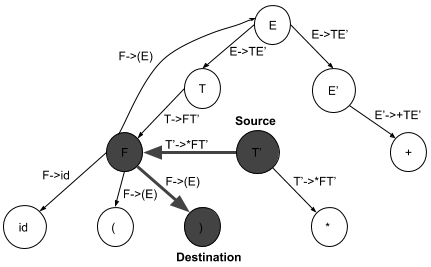
\includegraphics[width=0.8\textwidth]{Path2.png}
\caption{Path in the tree from T' to )}
\label{fig:Path 2}
\end{figure}

As T' is on top of the stack, it is popped from the stack and the outgoing edge from T' on the path is pushed on to the stack in reverse order. Same procedure, as described above, is applied on further steps.
\begin{center}
\begin{tabular}{ |c|c| } 
 \hline
 \textbf{stack} & \textbf{input string} \\
 \hline
 \$E'T'F* & id \\
 \$E'T'F & id * \\
 \$E'T')E( & id * \\
 \$E'T')E &	id * ( \\
 \$E'T')E'T & id * ( \\
 \$E'T')E'T'F &	id * ( \\
 \$E'T')E'T'id & id * ( \\
 \$E'T')E'T' & id * ( id \\
 \$E'T')E'$\epsilon$ & id * ( id \\
 \$E'T')E' & id * ( id \\
 \$E'T')$\epsilon$ & id * ( id \\
 \$E'T') & id * ( id \\
 \$E'T' & id * ( id ) \\
 \$E'$\epsilon$ & id * ( id ) \\
 \$E' & id * ( id ) \\
 \$$\epsilon$ & id * ( id ) \\
 \$ & id * ( id ) \\
 \hline
\end{tabular}
\end{center}

Now we have reached the end of the stack and obtained the input string for the cell M[T][)] filled incorrectly by the user. This input string is then used to generate hint questions.

\end{example}

% input string generation
\begin{algorithm}
\caption{Input string generation for LL parsing table}
\label{algo:inputstr gen}
\begin{algorithmic}[1]
\Function{generate\textunderscore input\textunderscore string}{$G, N, t$}
\State (E,V,LABELS) = \Call{generate\textunderscore graph}{$G$}
\State MINRULES = \Call{minrules\textunderscore gen}{$G$}
\State S := start symbol for G
\State SHORTEST = \Call{djikstra}{$E,V,S$}
\State PATH = SHORTEST[N] \Comment shortest path from S to N
\State STACK = \{\$S\}
\State PARTIAL = ""
\State (STACK,PARTIAL) = \Call{find\textunderscore input}{$PARTIAL, PATH, LABELS, MINRULES, G, STACK$}
\State SH = \Call{djikstra}{$E,V,N$}
\State PH = SH[t] \Comment shortest path from N to t
\State (STACK,PARTIAL) = \Call{find\textunderscore input}{$PARTIAL, PH, LABELS, MINRULES, G, STACK$}
\State INPUTSTRING = \Call{empty\textunderscore stack}{$G, STACK, PARTIAL, MINRULES$}
\State \Return INPUTSTRING
\EndFunction
\end{algorithmic}
\end{algorithm}

\begin{algorithm}
\caption{Generate partial input string}
\label{algo:find input}
\begin{algorithmic}[1]
\Function{find\textunderscore input}{$PARTIAL, PATH, LABELS, MINRULES, G, STACK$}
\State NT := set of all non-terminals in G
\While{PATH !empty}	
\State next = \Call{next}{$PATH$}
\State top = \Call{pop}{$STACK$}
\If{top = next}
\State dest = \Call{successor}{$PATH, next$}
\State label = \Call{reverse}{$LABELS[(next,dest)]$}
\State \Call{push}{$STACK, label$}
\Else
\If{top\in NT}
\State minr = \Call{reverse}{$MINRULES[top]$} \Comment reverses the minimum length rule for top
\State \Call{push}{$STACK, minr$}
\Else
\State PARTIAL = \Call{append}{$PARTIAL, top$} 
\EndIf
\EndIf
\EndWhile
\State \Return (STACK, PARTIAL)
\EndFunction
\end{algorithmic}
\end{algorithm}

\begin{algorithm}
\caption{Empty stack and generate final input string}
\label{algo:stack empty}
\begin{algorithmic}[1]
\Function{empty\textunderscore stack}{$G, STACK, PARTIAL, MINRULES$}
\State NT := set of all non-terminals in G
\While{\Call{top}{$STACK$}\neq \$}
\State top = \Call{pop}{$STACK$}
\If{top\in NT}
\State minr = \Call{reverse}{$MINRULES[top]$} \Comment reverses the minimum length rule for top
\State \Call{push}{$STACK, minr$}
\Else
\State PARTIAL = \Call{append}{$PARTIAL, top$} 
\EndIf				
\EndWhile
\State \Return PARTIAL
\EndFunction
\end{algorithmic}
\end{algorithm}

\begin{algorithm}
\caption{Generate minimum length rules for each non-terminal in grammar}
\label{algo:minrule gen}
\begin{algorithmic}[1]
\Function{minrules\textunderscore gen}{$G$}
\State RULES := table containing rules for every non-terminal in G
\State N := set of all non-terminals in G
\State MINRULES := table containing all minimum length rules of every n\in N
\ForAll{n in N}
\State R = RULES[n] \Comment set containing all rules of n
\State Rm = \Call{min}{$R$}
\State MINRULES[n] = Rm
\EndFor
\State \Return MINRULES
\EndFunction
\end{algorithmic}
\end{algorithm}

\begin{algorithm}
\caption{Graph generation from grammar}
\label{algo:graph gen}
\begin{algorithmic}[1]
\Function{generate\textunderscore graph}{$G$}
\State RULES := table containing rules for every non-terminal in G
\State N := set of non-terminals in G
\State T := set of terminals in G
\State V = N\cup T \Comment set of vertices in graph
\State E = \{\} \Comment set of edges in graph
\State LABELS := table with keys belonging to E
\ForAll{n in N}
\State R = RULES[n]
\State DEST = \{\}
\ForAll{rule in R}
\ForAll{symbol in rule}
\State DEST = DEST\cup \{symbol\}
\State E = E\cup (n,symbol)
\If{$LABELS[(n,symbol)] = null \parallel \Call{length}{rule} < \Call{length}{LABELS[(n,symbol)]}$}
\State LABELS[(n,symbol)] = rule
\EndIf
\EndFor
\EndFor
\EndFor
\State \Return (E,V, LABELS)
\EndFunction
\end{algorithmic}
\end{algorithm}

% end input string generation

\subsection{LL Parsing Moves}
\label{subsec:llmoves}

This sub-domain of problems attempts to teach users how to parse an input string using the LL parsing table for the corresponding grammar. The problems in this sub-domain involve predicting the next move in a sequence of parsing moves. The algorithms specific to this domain of problems include preprocessing, primary problem generation and hint question generation. The procedure for preprocessing is shown in algorithm \ref{algo:preprocessing-llmoves}. Primary problem generation involves questions that are of the MCSA type. This is shown in algorithm \ref{algo:primary-llmoves}. Hint questions H1 and H2 are generated using the procedure described in algorithm \ref{algo:hint-llmoves}.

\begin{algorithm}
\caption{Preprocessing for LL parsing moves}
\label{algo:preprocessing-llmoves}
\begin{algorithmic}[1]
\Function{preprocess\textunderscore llmoves}{$G, L, s$}
\State I := Valid input string for parsing with \$ at the end
\State M := sequence of moves of parsing on input string
\State STACK := stack containing \$ and s, with s on top
\State index = 0    \Comment move number
\While{\Call{top}{STACK}\neq \$}
\State move = llmove[I]
\State M[index] = move
\State index = index + 1
\EndWhile
\State r := random number on index of moves
% \State move = M[r]
% \State S := data structure for moves
% \State S[0] = M[r]
% \State index = 1    \Comment move number
% \While{M !empty}
% \State S[index] = M[r+index]
% \EndWhile
\State \Return (M, r)
\EndFunction
\end{algorithmic}
\end{algorithm}

\begin{algorithm}
\caption{Primary problem generation for LL parsing moves}
\label{algo:primary-llmoves}
\begin{algorithmic}[1]
\Function{generate\textunderscore primary\textunderscore question\textunderscore llmoves}{$context$}
\State S := M[0] to M[r]
\State Q := S, "What will be the next move?"
\State index := move number
\State F = M[index]
\State \Return (Q, F)
\EndFunction
\end{algorithmic}
\end{algorithm}

\begin{algorithm}
\caption{Hint question generation for LL parsing moves}
\label{algo:hint-llmoves}
\begin{algorithmic}[1]
\Function{generate\textunderscore hint\textunderscore question\textunderscore llmoves}{$choice, type$}
\If{type = 1}
\State H := "By which of the following rule, do you think choice should be the next move? 1. If X = a = \$, ..... 4. No valid rule."
\If{choice$\in$ I}
\State A := 4
\ElsIf{choice$\in$ C}
\State A := 1 or 2 or 3
\EndIf
\ElsIf{type = 2}
\State H := "Probably context should be the next move. What do you think ?"
\State A := "Yes"
\EndIf
\State \Return (H, A)
\EndFunction
\end{algorithmic}
\end{algorithm}

\section{SLR Parsing}
\label{slrparsing}

This domain of problems attempts to teach the SLR parsing technique to users. The types of questions covered in this domain include filling up entries in certain data structures. This domain is further divided into sub-domains: SLR canonical set, SLR parsing table and SLR parsing moves. These are described in the subsections that follow. 

\subsection{SLR Canonical Set}
\label{subsec:slrcanonical}

SLR canonical sets have been described in section \ref{para:Canonical Set} of chapter \ref{chap:background}. Questions are generated on concepts involving item sets (described in \ref{para:Canonical Set}). These questions involve filling up entries in these  item sets and choosing correct item sets for a particular context. These questions are divided into two categories - SLR closure and SLR goto.

\subsubsection{SLR Closure}
\label{ssec:slrclosure}
SLR Closure of an item set have been described in section \ref{} of chapter \ref{}. This is used in building SLR canonical set. This domain 

\subsubsection{SLR GOTO}
\label{ssec:slrgoto}

The two types of questions generated are distinguished on the basis of levels. They are described below:
\begin{itemize}
\item \textbf{Level 1:}
\item \textbf{Level 2:}
\end{itemize}

\subsection{SLR Parsing Table}
\label{subsec:slrtable}

\subsection{SLR Parsing Moves}
\label{subsec:slrmoves}

\begin{algorithm}
\caption{}
\label{algo:}
\begin{algorithmic}[1]
\Function{}{}
\EndFunction
\end{algorithmic}
\end{algorithm}

We have used three types of questions as described in chapter \ref{chap:overview}, out of which, Question 1 is the primary question and Questions 2 and 3 are hint questions of type 1 (H1) and 2 (H2) respectively. These questions are used for all the parsing techniques. However in some techniques, different types of questions are added by creating levels in them.

As an example, consider the LL parsing technique. In the LL Parsing table, we have created two levels: Level 1 uses the same flow as described, but level 2 uses the input strings generated by the tool for wrongly entered cells (in the hint questions). Primary questions remain the same for both levels. The algorithm for level 2 is described in section \ref{sec:LL Table Level 2}.

Similarly for the GOTO function of SLR Canonical set, we have created two levels: Level 1 uses the same algorithm described below. However for level 2, there is a change in the type of questions generated and hence the algorithm is different. The algorithm for level 2 of GOTO is described in section \ref{sec:Goto Level 2}.

\begin{algorithm}                     
\begin{algorithmic} [1]
\If{stack is not empty}, 
\State Take one value out of the stack.
\If{state is 1}
\If{answer is not null}
\State Separate the incorrect options from the answer.
\State Also find the correct options which are not marked as the answer.
\If{there are no incorrect options and left out correct options}
\State assign answer = null and go to step 4.
\Else
\State Assign state = 2 and answer = null.
\EndIf
\Else
\State Display Question 1 and collect the marked options as answer.
\EndIf
\EndIf
\If{state is 2}
\If{answer is null or answer is right}
\If{there are incorrect options}
\State Pick one incorrect option
\State Display and take answer of Question 2 for this incorrect option.
\Else
\State Assign state = 4 and answer = null.
\EndIf
\Else
\State Display and take answer of Question 2 for the current incorrect option.
\EndIf
\EndIf
\If{state is 4}
\If{answer is null or answer is right}
\If{there are correct options which were left out in the answer}
\State Take one correct option and assign state = 3.
\Else
\State Assign state = 1, answer = null
\State Display Question 1 and collect the marked options as answer.
\EndIf
\Else
\State Display and take answer of Question 2 for the current incorrect option.
\EndIf
\EndIf
\If{state is 3}
\If{answer is right}
\State Assign state = 4
\State Display and take answer of Question 2 for the current correct option.
\Else
\State Display and take answer of Question 3 for the current correct option.
\EndIf
\EndIf
\EndIf
\end{algorithmic}
\end{algorithm}

\section{Level 2 of GOTO in SLR Canonical Set}
\label{sec:Goto Level 2}
In SLR Canonical set, choice for CLOSURE and GOTO function is given to generate questions on them. Different kinds of question are added for GOTO function by creating another level in it.

In this level of GOTO, we have again used three types of questions. But the content of the questions is different here. Question 1, which is the main question, contains the reverse question of the one in level 1 of GOTO. Question 2 and 3 are the hint questions but with different content.
\begin{example}
For the grammar used in \ref{ex:First}, questions are of the form:
\begin{itemize}
\item \textbf{Question 1 (Main Question):} In GOTO(I, X), if X is the grammar symbol E, then which of the following itemsets can act as I to get itemset {[E' $\to$ +E.]} as result ?

\textbf{Options:}

I0: T $\to$ .1 \quad E'' $\to$ .E \quad T $\to$ .0 \quad E $\to$ .TE'

I1: E $\to$ T.E' \quad E' $\to$ . \quad E' -> .+E

I2: T $\to$ 1.

I3: T $\to$ 0.

I4: E'' $\to$ E.

I5: T $\to$ .0 \quad E $\to$ .TE' \quad E' $\to$ +.E \quad T $\to$ .1

I6: E $\to$ TE'.    

I7: E' $\to$ +E.

\item \textbf{Question 2 (Hint Question, type 1):} Should GOTO(I, X), where I is the itemset containing {[T $\to$ .0], [T $\to$ .1], [E $\to$ .TE'], [E'' $\to$ .E]} and X is the symbol E, result in the itemset {[E' $\to$ +E.]} ?  

\textbf{Options:} Yes \quad No

\item \textbf{Question 3 (Hint Question, type 2):} What is the GOTO of itemset {[T $\to$ .0], [T $\to$ .1], [E $\to$ .TE'], [E'' $\to$ .E]} on symbol E ?

\textbf{Options:} E $\to$ .TE' \quad E' $\to$ .+E \quad T $\to$ 1. \quad T $\to$ 0. \quad E'' $\to$ E. \quad T $\to$ .1 \quad E $\to$ TE'. \quad E' $\to$ +E.
\end{itemize}
\end{example}

We have used 4 states again here to signify the type of question to be asked and the value for which it is asked.
\begin{itemize}
\item \textbf{State 1} signifies that the main question is to be asked for one of the itemsets.
\item \textbf{State 2} signifies that the hint question of type 1 is to be asked for one of the incorrect options marked by the user.
\item \textbf{State 3} signifies that the hint question of type 2 is to be asked for same incorrect option used in state 2.
\item \textbf{State 4} signifies that the hint question of type 1 is to be asked for one of the correct options left by the user from marking.
\end{itemize}
The algorithm below describes the scenario:
\begin{algorithm}
\caption{Reverse Problem Generation}
\label{algo:Reverse Problem Generation}

\begin{algorithmic}[1]
\Require Grammar
\State Initialise state = 1 and answer = null. 
\State Four random numbers are generated on the values which are the output of the technique chosen. These random numbers are used as index of the values.
\State A stack containing the values, corresponding to random numbers, for which questions are to be asked.
\algstore{rev prob gen}
\end{algorithmic}
\end{algorithm}

\begin{algorithm}                     
\begin{algorithmic} [1]
\algrestore{rev prob gen}
\If {stack of values is not empty}, 
\State Take one value out of the stack.
\If{state is 1}
\If{answer is not null}
\State Separate the incorrect options from the answer.
\State Also find the correct options which are not marked as the answer.
\If{there are no incorrect and left out correct options}
\State answer = null
\State Go to step 4.
\Else
\State Assign state = 3 and answer = null.
\EndIf
\Else
\State Display Question 1 and collect the marked options as answer.
\EndIf
\EndIf
\If{state is 3}
\If{answer is null or answer is right}
\If{there are no incorrect options}
\State Assign state = 4 and answer = null.
\Else
\State Take one incorrect option and assign state = 2.
\EndIf
\Else
\State Display and take answer of Question 3 for the current incorrect option.
\EndIf
\EndIf
\If{state is 2}
\If{answer is right}
\State Assign state = 3.
\State Display and take answer of Question 3 for the current incorrect option.
\Else
\State Display and take answer of Question 2 for the current incorrect option.
\EndIf
\EndIf
\If{state is 4}
\If{answer is null or answer is right}
\If{there are correct options left}
\State Pick 1 value from correct options.
\State Display and take answer of Question 2 for the current correct option.
\Else
\State Assign state = 1 and answer = null.
\State Display Question 1 and collect the marked options as answer.
\EndIf
\EndIf
\EndIf
\EndIf
\end{algorithmic}
\end{algorithm}

\chapter{Interface}
\label{chap:interface}

The tool developed in this thesis works as a console application. This tool can also be merged with other interfaces easily. We have developed a file, named as QuestionGenerator.java, which is the main file in the tool, to handle the other parts of the system.

There is another file in the tool called as QuestionSet.java which contains the recursive functions. These functions are called by the function in QuestionGenerator.java.

To merge the tool with Web Interface, one has to merge these two files into one file, say in QuestionGenerator.java. This is required because  HTTP is stateless protocol so cannot handle the recursive functions. The resultant file, QuestionGenerator.java, can then be called by the controller of the system to perform the necessary operations.

There is one more file, QuestionFormat.java. As HTTP is stateless and we cannot store data, so the object of this file can be used to pass data to the server. While merging with web interface, another file of same kind will be required to pass updated data back. In this, these two files can be used to pass data to and fro.

\section{Detailed Explanation of the Files in the Tool}
\subsection{QuestionGenerator.java}
This file is required to perform the preprocessing step described in section \ref{subsec:preprocessing}. The function in this file calls the functions in QuestionSet.java for other steps. Grammar is taken as input from the user in the function in QuestionGenerator.java. Then First set, Follow set, LL Parsing Table, LL Parsing Moves, SLR Canonical set, SLR Parsing Table and SLR Parsing Moves are calculated based on the choice for which questions are to be generated. Random numbers are also generated in this function for some techniques. These random numbers are used to select values for which questions are to be generated.

This function calls another function in a separate java file to generate input strings for wrong entered cells of LL Parsing Table. These input strings are then used in hint questions for LL Parsing Table. There are two choices of levels for some techniques. This choice is taken from user in this function, according to which, certain set of questions are generated in next steps.

\subsection{QuestionSet.java}
There are various functions in this file. All of them are recursive functions. These functions call the functions of core engine to perform other steps such as main problem generation, answer evaluation and hints generation of the tool. The termination condition in these functions decide the end of program. These functions are also used to display question, which it obtains from core engine and take answer of that question, which it pass to the core engine for evaluation.

\subsection{QuestionFormat.java}
All the data, which is required by the system, to pass to the server (if merged to web interface), is contained in this file. The system uses the object of this class to pass data to and fro. As the problems are dynamically generated in the system, so the amount of information required to be passed is also huge. Therefore, this file contains a lot of variables which represent different kinds of information.
\chapter{An interactive walk through the tool}
\label{interactions}

This chapter walks through some interactions with the tool. Design and implementation of the tool was discussed in chapter \ref{chap:overview} and \ref{chap:algorithms}. Instances of the tool's response to specific input and user stimuli are shown here.

A sample text file containing a CFG is passed as an argument to the tool. The grammar is shown in figure \ref{fig:grammar}. This grammar used as a basis for generating questions. Upon receiving this grammar as input, the tool displays a menu to the user asking her to choose the domain for which problems are to be asked. This is shown in figure \ref{fig:main-menu}. Based on this choice, a primary problem is generated for one of the values in the data structure generated during preprocessing. These values are basically the non-terminals in the grammar. This primary problem is shown in figure \ref{fig:primary-ques}. As shown in the image, the question was asked about the first set of a non-terminal in the grammar. The user fills some options as the solution to the problem. As the answer is correct for the above question, then next primary question is generated for the next non-terminal. This is shown in figure \ref{fig:primary-correct}.

However, if the answer is wrong then the tool generates hint questions. In this case, the user enters a set of options (id, *) out of which there is an incorrect option (according to grammar, First[F] is \{id, (\}). Here the tool generates a hint question of type 1 (H1), for each wrong option selected. Since there is one such wrong option (*), the tool generates a hint question (H1) for it. Figure \ref{fig:hint-h1} shows this scenario. 

Now, if the answer to this question is wrong, then system generates this same question repeatedly, until it gets the right answer. This is shown in figure \ref{fig:hint-repeat}. If the user now answers this question correctly, the tool generates a hint question of type 2 for the correct option left unmarked. Figure \ref{fig:hint-h1-h2} shows this scenario.

\begin{figure}
\centering
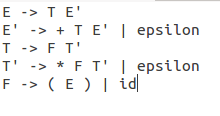
\includegraphics[width=0.8\textwidth]{grammar.png}
\caption{A Context Free Grammar given as input}
\label{fig:grammar}
\end{figure}

\begin{figure}
\centering
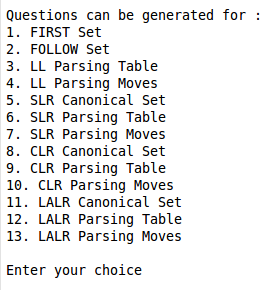
\includegraphics[width=0.8\textwidth]{menu.png}
\caption{A main menu showing the possible domains for which problems can be generated}
\label{fig:main-menu}
\end{figure}

\begin{figure}
\centering
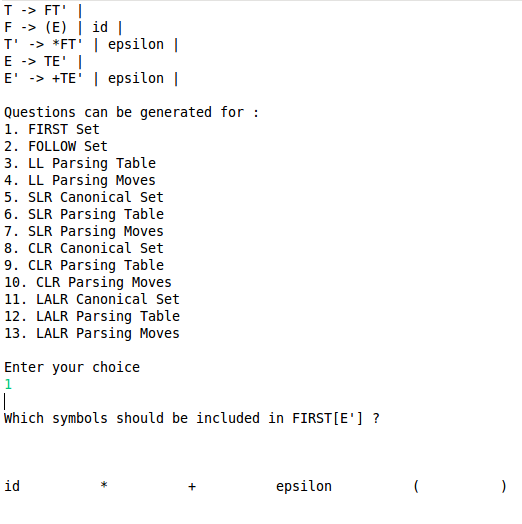
\includegraphics[width=0.8\textwidth]{PrimaryQuestion.png}
\caption{Primary question asked by the tool}
\label{fig:primary-ques}
\end{figure}

\begin{figure}
\centering
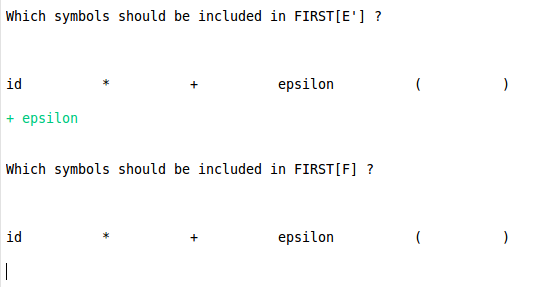
\includegraphics[width=0.8\textwidth]{NextPrimaryQ.png}
\caption{Tool's response to a correct answer by the user}
\label{fig:primary-correct}
\end{figure}

\begin{figure}
\centering
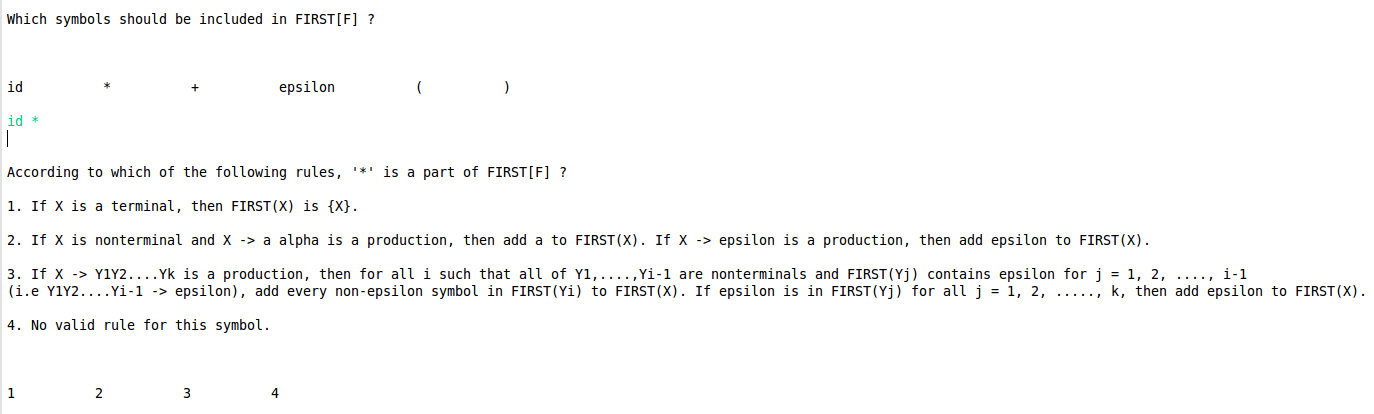
\includegraphics[width=0.8\textwidth]{Type1Incorrect.png}
\caption{Hint question of type 1 generated for incorrect option}
\label{fig:hint-h1}
\end{figure}

\begin{figure}
\centering
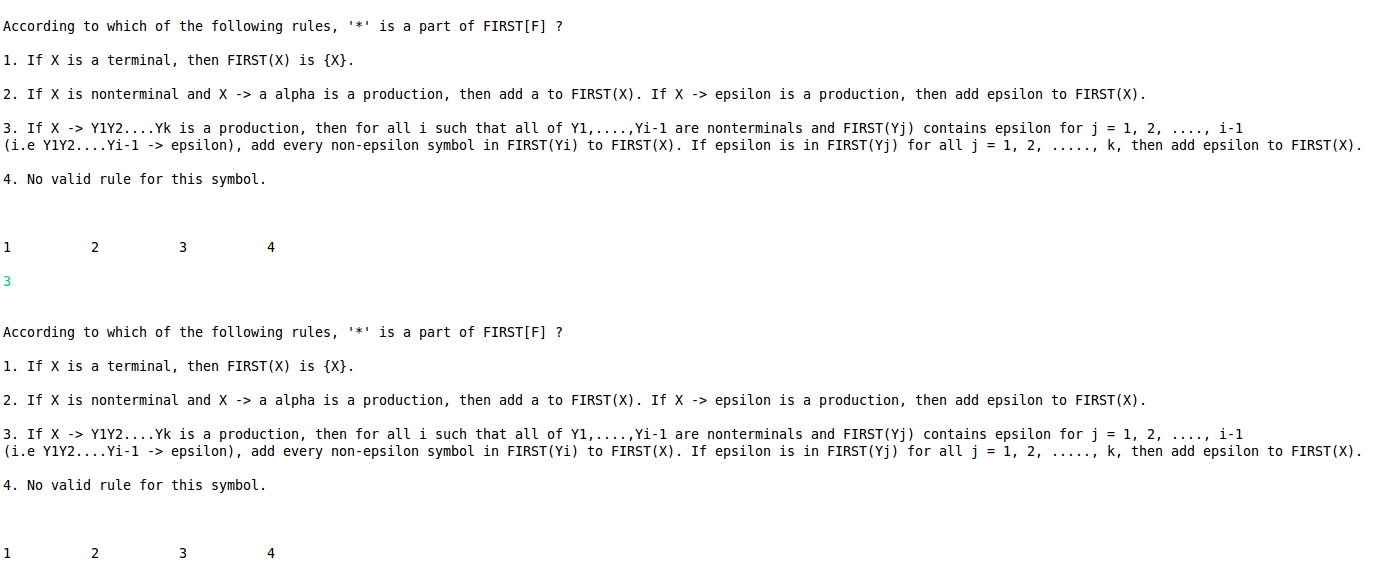
\includegraphics[width=0.8\textwidth]{Type1IncorrectRepeat.png}
\caption{Repetition of hint question due to incorrect attempt}
\label{fig:hint-repeat}
\end{figure}

\begin{figure}
\centering
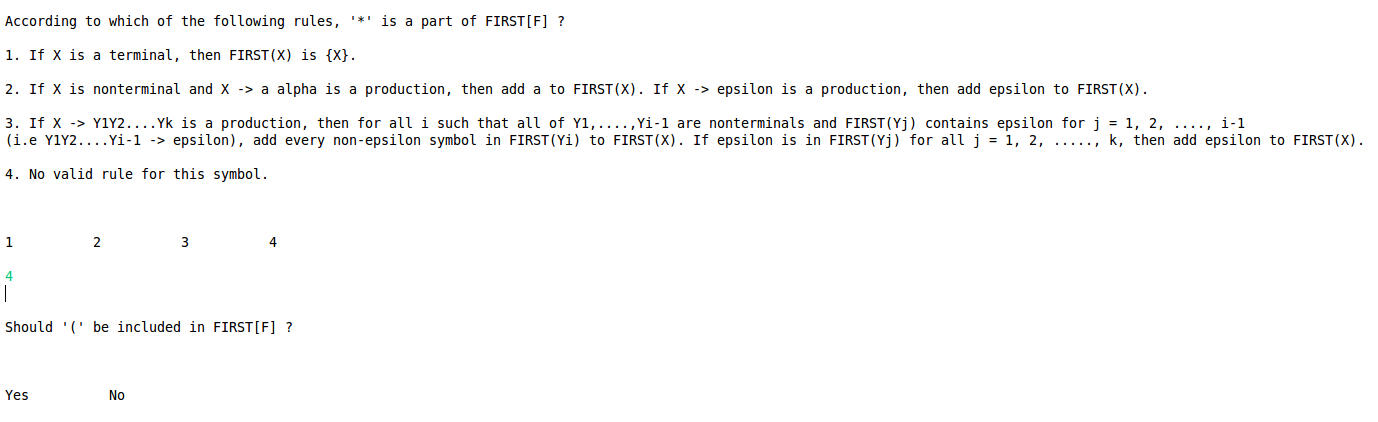
\includegraphics[width=0.8\textwidth]{Type2Correct.png}
\caption{H2 generated when user answers correctly}
\label{fig:hint-h1-h2}
\end{figure}

Again, if the user marks wrong option, then it generates the same question until she choose the right option.

\begin{figure}
\centering
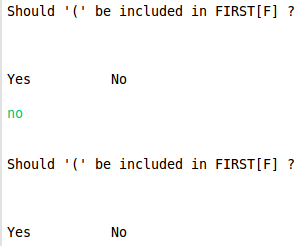
\includegraphics[width=0.8\textwidth]{Type2CorrectRepeat.png}
%\caption{Tree after applying Dijkstra Algorithm second time}
%\label{fig:Dijkstra Tree 2}
\end{figure}

After receiving the correct answer for previous question, the tool generates hint question of type 1 for this correct option. This question asks about the rule by which this value must be a part of correct answer for the primary question.

\begin{figure}
\centering
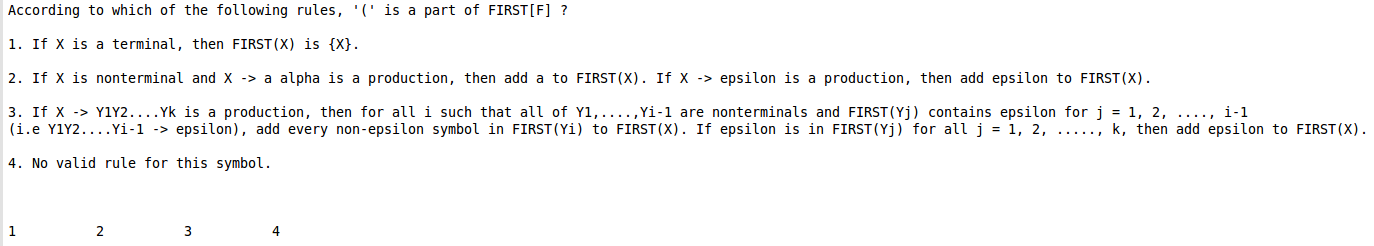
\includegraphics[width=0.8\textwidth]{Type1Correct.png}
%\caption{Tree after applying Dijkstra Algorithm second time}
%\label{fig:Dijkstra Tree 2}
\end{figure}

Again, if the rule marked is wrong, then the tool repeats the question, until correct rule is received.

\begin{figure}
\centering
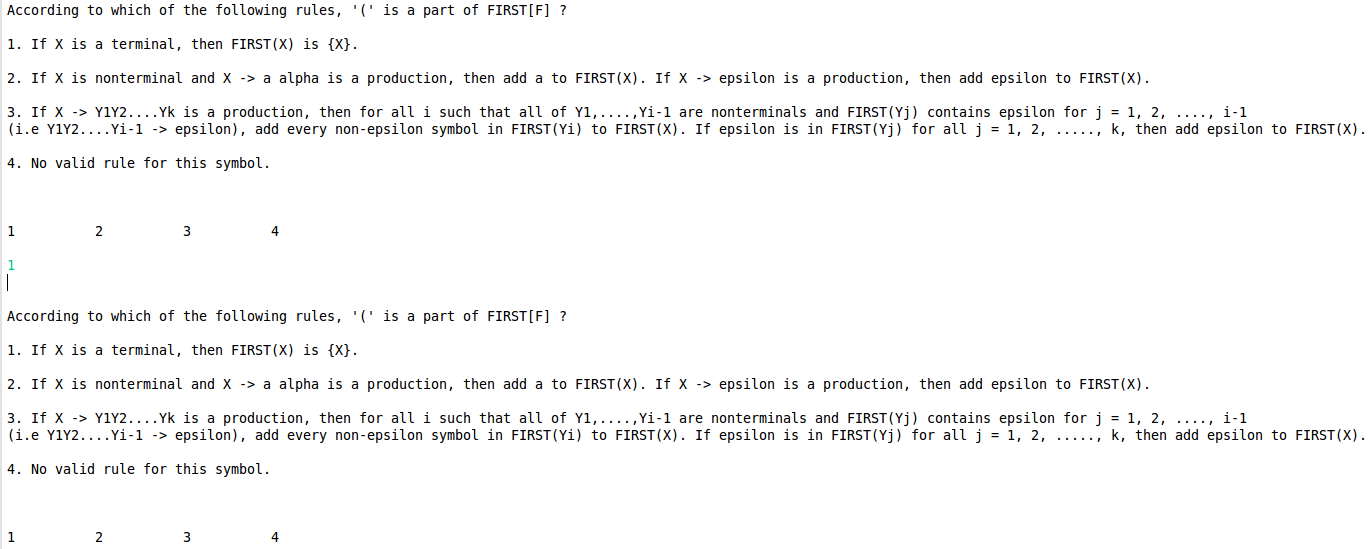
\includegraphics[width=0.8\textwidth]{Type1CorrectRepeat.png}
%\caption{Tree after applying Dijkstra Algorithm second time}
%\label{fig:Dijkstra Tree 2}
\end{figure}

On getting right answer to the above hint question, the tool again generates the same primary question, to check whether the user understands the solution for the question well or not.

\begin{figure}
\centering
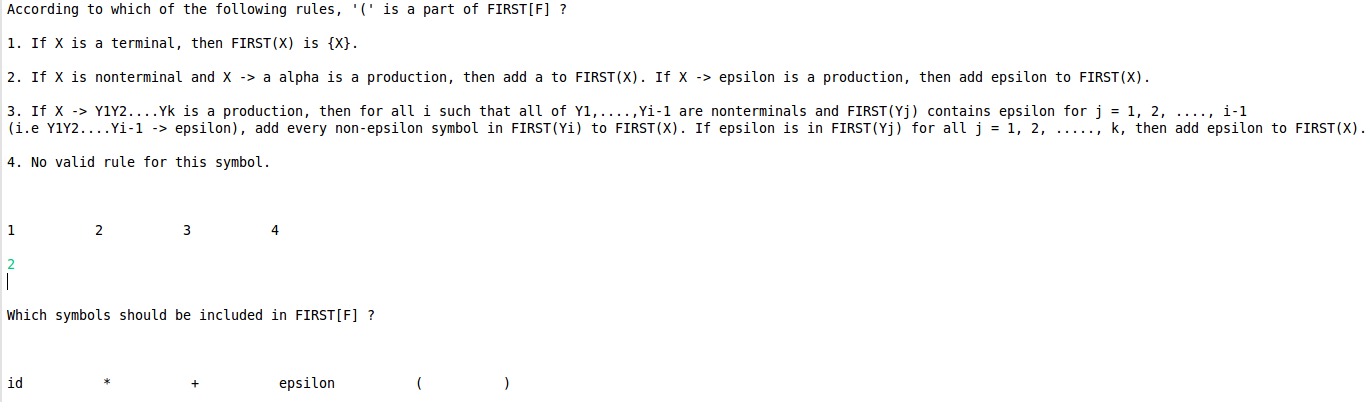
\includegraphics[width=0.8\textwidth]{PrimaryQRepeat.png}
%\caption{Tree after applying Dijkstra Algorithm second time}
%\label{fig:Dijkstra Tree 2}
\end{figure}

If this time, the user gives the right answer, then next primary question is generated. Otherwise, the process repeats, until the tool obtains the right answer of the primary question from the user.

\begin{figure}
\centering
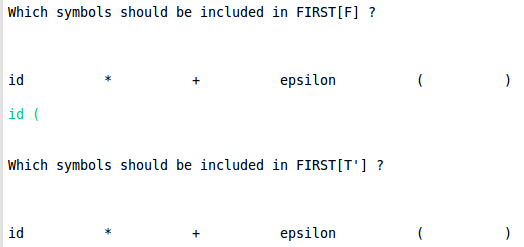
\includegraphics[width=0.8\textwidth]{NewPrimaryQ.png}
%\caption{Tree after applying Dijkstra Algorithm second time}
%\label{fig:Dijkstra Tree 2}
\end{figure}

The process is repeated for the rest of the values.

\section{Level 2 of LL Parsing Table}
The primary question, for this level of LL Parsing Table, remains same as in level 1 of LL Parsing Table. 

\begin{figure}
\centering
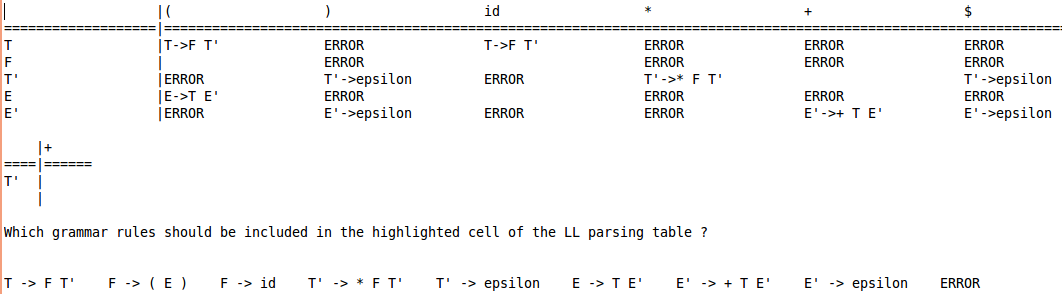
\includegraphics[width=0.8\textwidth]{llTableL2Primary.png}
%\caption{Tree after applying Dijkstra Algorithm second time}
%\label{fig:Dijkstra Tree 2}
\end{figure}

Firstly, it asks primary questions for all the values.
\begin{figure}
\centering
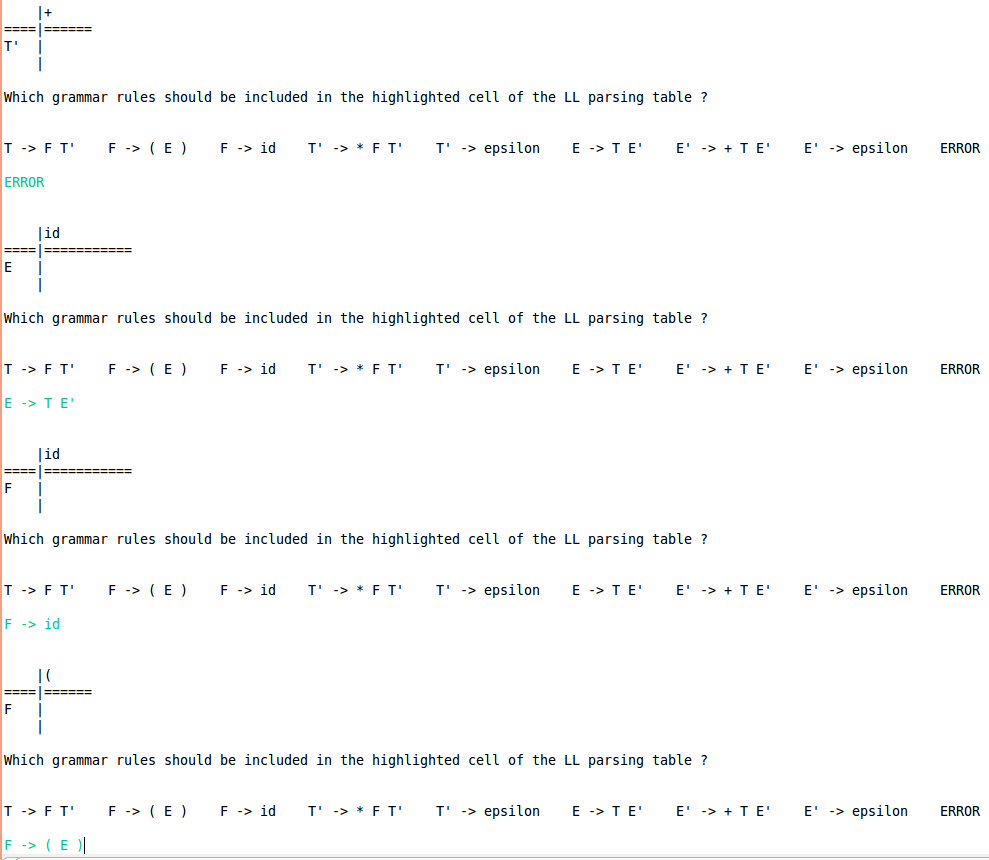
\includegraphics[width=0.8\textwidth]{LLlevel2Primary.png}
%\caption{Tree after applying Dijkstra Algorithm second time}
%\label{fig:Dijkstra Tree 2}
\end{figure}

Then it generates hint questions for all the cells in which user has filled wrong entry. But there is a change in the hint questions. For hints, the tool automatically calculates an input string for the cell, in which user has filled wrong entry. The tool parses this input string, using the LL Parsing table filled by the user. Then in the hint question, the tool shows the moves of the parser on this input string and ask the user to fill the cell again.
\begin{figure}
\centering
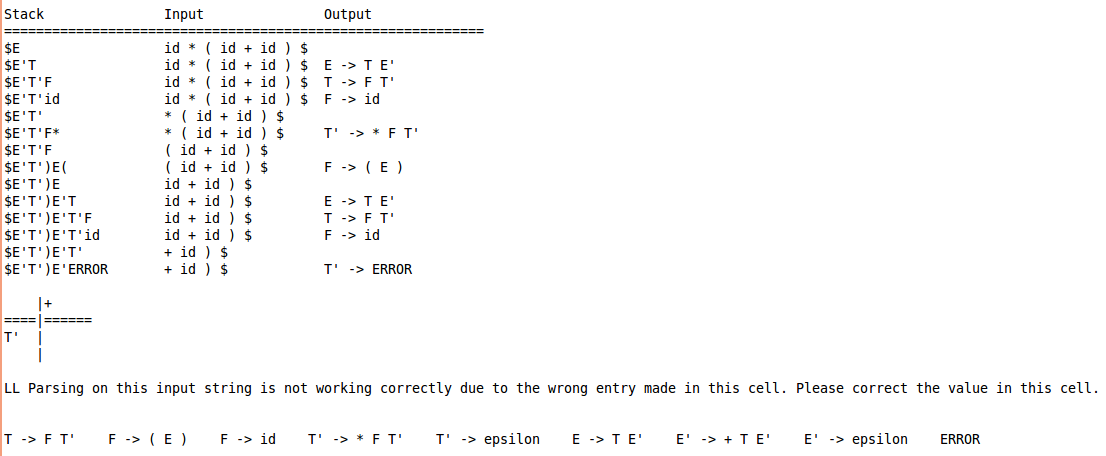
\includegraphics[width=0.8\textwidth]{Level2Hint.png}
%\caption{Tree after applying Dijkstra Algorithm second time}
%\label{fig:Dijkstra Tree 2}
\end{figure}

\section{Level 2 of GOTO}
In level 2 of GOTO function, format of primary problem is the reverse of those in level 1.
\begin{figure}
\centering
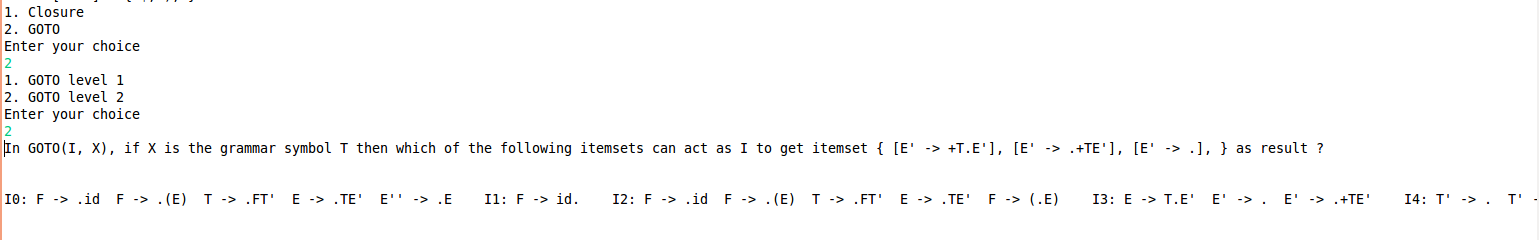
\includegraphics[width=0.8\textwidth]{Level2GOTOPrimary.png}
%\caption{Tree after applying Dijkstra Algorithm second time}
%\label{fig:Dijkstra Tree 2}
\end{figure}

The content of hint questions and their sequence is a little different. Two questions are asked for each wrong option selected and 1 question for each right answer left unmarked in solution. H1 and H3 are of similar type.
H1 for incorrect:
\begin{figure}
\centering
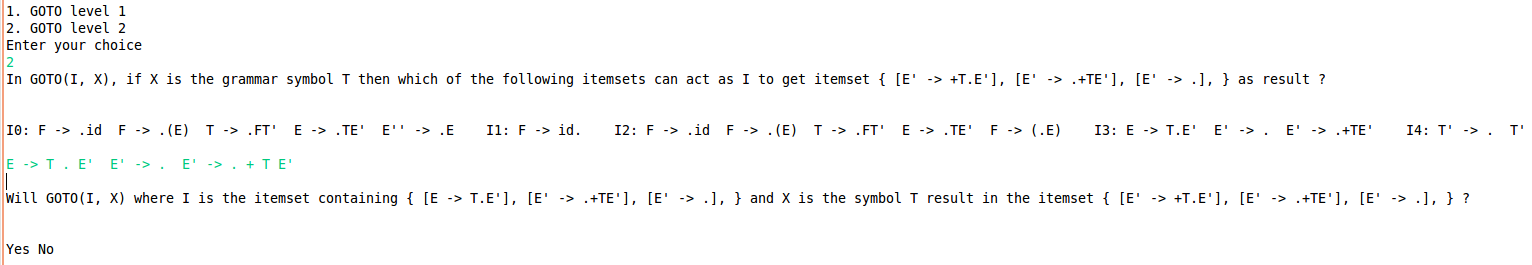
\includegraphics[width=0.8\textwidth]{Level2GotoH1.png}
%\caption{Tree after applying Dijkstra Algorithm second time}
%\label{fig:Dijkstra Tree 2}
\end{figure}

H2 for same incorrect,
\begin{figure}
\centering
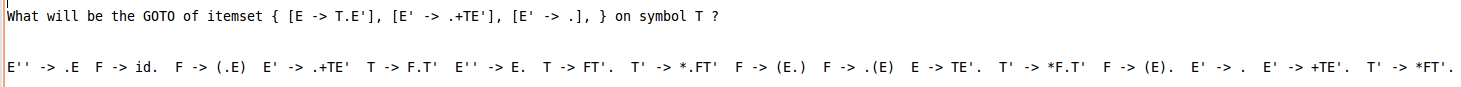
\includegraphics[width=0.8\textwidth]{Level2GotoH2.png}
%\caption{Tree after applying Dijkstra Algorithm second time}
%\label{fig:Dijkstra Tree 2}
\end{figure}

H3 for correct one(or H1 for correct),
\begin{figure}
\centering
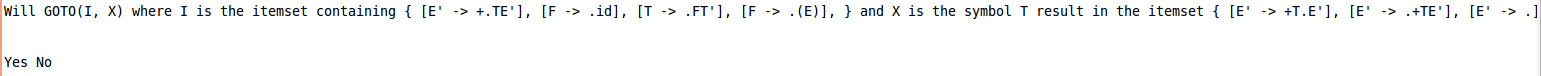
\includegraphics[width=0.8\textwidth]{Level2GotoH3.png}
%\caption{Tree after applying Dijkstra Algorithm second time}
%\label{fig:Dijkstra Tree 2}
\end{figure}
\chapter{Related work}
\label{chap:related}

Computer-based Education systems have been in existence for quite a long time. The LISA tool \cite{mernik2003educational} founded by Marjan Mernik and Viljem Zumer, helps students in learning compilers through animations and visualizations. The tool is built for 3 phases of compiler - lexical analysis, syntax analysis and semantic analysis. For learning lexical analysis, animation is done in DFAs. Similarly, for syntax analysis, animation in construction of the synatx tree and for semantic analysis, animation in the node visits of the semantic tree and evaluation of attributes in the semantic tree is done.

\chapter{Conclusions and Future Work}
\label{chap:conclusion}
Online Tutoring System for Compilers is an automated system to help students in learning process. It takes CFG as input. Using the grammar, it determines the results of various parsing techniques. Based on these results, the tool generates questions automatically. If the answer is correct, it generates the next problem, otherwise, it generates hint questions to reach to the correct solution of the problem. It generates different type of hint questions.

Various challenges occur in developing the tool, which are listed as follows:
\begin{enumerate}
\item Generation of input string for the cells of SLR Parsing table, which can be used in hint questions for the incorrectly entered cells of parsing table.
\item The tool is not developed for other parsing techniques such as CLR, LALR.
\item The tool has been developed only for the parsing phase of Compiler.
\end{enumerate}

Future work include the improvement of this tool. Some of them are listed below:
\begin{enumerate}
\item Generation of input string for the cells of SLR Parsing table is in progress.
\item Develop the tool for other parsing techniques such as CLR, LALR.
\item Develop tools for other phases of Compiler and merge them into a single tool.
\end{enumerate}

\begin{singlespace}
\cleardoublepage
\phantomsection \label{listoffig}
\addcontentsline{toc}{chapter}{References}
\renewcommand\bibname{References}
\printbibliography
\nocite{*}
\end{singlespace}

\end{document}
